\documentclass[11pt]{article}
\usepackage{graphicx}
\usepackage{amssymb}
\usepackage{epstopdf}
\usepackage{amsfonts}
\usepackage{natbib}
\usepackage{subfigure}
\usepackage{pdfsync}
\usepackage{xspace}
\usepackage{color}
\usepackage{rotating}

%% some handy things for making bold math
\def\bm#1{\mathpalette\bmstyle{#1}}
\def\bmstyle#1#2{\mbox{\boldmath$#1#2$}}
\newcommand{\thh}{^\mathrm{th}}


%% Some pretty etc.'s, etc...
\newcommand{\cf}{{\em cf.}\xspace }
\newcommand{\eg}{{\em e.g.},\xspace }
\newcommand{\ie}{{\em i.e.},\xspace }
\newcommand{\etal}{{\em et al.}\ }
\newcommand{\etc}{{\em etc.}\@\xspace}



%% the page dimensions from TeXShop's default---very nice
\textwidth = 6.5 in
\textheight = 9 in
\oddsidemargin = 0.0 in
\evensidemargin = 0.0 in
\topmargin = 0.0 in
\headheight = 0.0 in
\headsep = 0.0 in
\parskip = 0.2in
\parindent = 0.0in


\title{Variation in Parentage-Based Tagging \\
and Coded-Wire  Tagging  Rates}
%\author{Eric C. Anderson\thanks{
%    Fisheries Ecology Division, 
%    Southwest Fisheries Science Center, 
%    110 Shaffer Road,
%    Santa Cruz, CA 95060}
%}
\begin{document}

\maketitle


\begin{abstract}
Realized rates of tagging are investigated for scenarios using parentage-based tagging (PBT)
and coded wire tags (CWT).  
Using CWTs the fraction of fish tagged can usually be accurately
estimated at the time of tagging/release, though there will be some variation in the realized
proportion of tagged versus untagged fish at the time of adult sampling.  In a PBT
scenario, the {\em expected} fraction of fish tagged at the time of tagging can be
estimated from the number of successfully-genotyped families that
contributed to the release group.  However, unless 100\% of the families producing the release
group are successfully genotyped, the realized PBT tagging rate can differ from the
expected rate because different families produce different numbers of offspring that survive
at different rates to time of tagging.  Additional variation is possible due to differential
survival of family groups to the time of adult sampling.  These issues, as well as their
consequences for the variance in the estimated expanded number of recoveries, are explored
through simulation.  The indicate that it is best to maintain a high ($>96\%$) fraction
of successfully-genotyped families, especially when the number of parents producing the release
group is small ($<20$) and the product of the sampling rate in the fishery
and the marking rate in the release group is high ($\geq 75\%$).

\end{abstract}


\tableofcontents

\section{Introduction}
We develop a simple system of simulations to describe, explore, and understand
variation in the realized tagging rates achieved when using parentage-based tagging (PBT)
or coded-wire tags (CWTs) for hatchery-raised salmon.  Here we describe simulation routines
and the assumptions made in them for both CWTs and PBT.  We subsequently investigate the effective
number of breeders in hatchery populations, and the distribution
of release group sizes, marking rates and fishery sampling rates to understand the potential
consequences of this tagging rate variation.

We pursue two (related) simulations.  In the first, we focus  exclusively on the
variance in the tagging rate itself.  In the second we also include fishery sampling
aspects to assess the practical importance of PBT tagging rate variation.

\section{Simulation 1. Tagging rate variation}

\subsection{Tagging rates of CWTs}
Coded wire tags are typically deployed
when fish are large enough to be tagged and to have their adipose fins clipped, frequently
just days before release.  In large hatchery programs, the tagging of release
groups may be undertaken with specialized tagging trailers that automate the tagging and marking
process and allow for a precise count of the number of fish tagged and marked,
as well as the total number of fish in the release group.  Within a release group, the tags are
assumed to be randomly assigned to individual fish, so there is no association between the family
the fish came from and whether or not it carries a tag.  For these simulations, we will assume
that the CWT tagging rate, $p_\mathrm{cwt}$, is known without error at the time of release and that
the rate of tag shedding has been accounted for in it. 

Most CWT recaptures occur in adult fish.  Each tagged fish at the time of recovery can be
expanded by $1/p_\mathrm{cwt}$ into an estimate of the total number of impacts that the tag recovery represents.
Usually, $p_\mathrm{cwt}$ will provide a good estimate of the fraction of adult fish from the release group
that are tagged at the time of recovery, a proportion we will call the {\em realized} tagged
fraction, $\tilde{p}_\mathrm{cwt}$.  It should be clear that the realized
tagged fraction is the relevant quantity when expanding
tag recoveries of adult fish, but is typically not known.  
We will assume that tagged and untagged fish have the same rate of
survival so that adult fish can be regarded as a random sample from the fish in the release group (hence,
we are not modeling the
effects of mark selective fisheries, etc.).
Although the sampling is technically without replacement, it is reasonable to model the sampling as
with replacement because so few adults survive from any given cohort.  For our simulations, if we consider the
$N_A$ adults that have survived from a release group tagged at rate $p_\mathrm{cwt}$  we will
model $\tilde{p}_\mathrm{cwt}$ as having a scaled binomial distribution:
$	\tilde{p}_\mathrm{cwt} \equiv X/N_A$ where 
\[
X \sim \mathrm{Binomial}(N_A, p_\mathrm{cwt}).
\]


\subsection{Tagging rates with PBT}
Determining expected and realized PBT tagging rates proceeds in a different fashion.  In PBT, the
offspring of a set of male and female spawners are raised separately in the hatchery
as a single release group. Let us assume that there are $S$ male-female pairs of spawners
whose eggs are contributed to the release group.  PBT will work most
efficiently with 100\% tagging---in other words, when all the parents of a release group
are genotyped.  However, there may be some rate at which genotypes are not obtained for certain
individuals.  Currently,
genotype data from both parents is  required for PBT; however, with newer genotyping
systems, that can economically provide more genotypes per individual, it will be possible
to accurately perform assignments of offspring to single parents.  Regardless of the exact mechanism,
we can still focus on the tagging rate of families (the offspring of two distinct parents) in the hatchery: under current practices
a family is tagged if both parents are genotyped; allowing single-parent assignments a family would be
considered tagged if at least one parent was genotyped.  For our 
simulations, we will let $G$ families out of $S$ be tagged.
Under this assumption, the
fraction of families that are PBT-tagged is,
\[
f_\mathrm{pbt} = \frac{G}{S}.
\]   
This quantity is the expected value of $p_\mathrm{pbt}$, the PBT tagging rate, defined to be the
fraction of juveniles in the release group that will be tagged at the time
of release.

 
  
Depending on how much information about spawning is recorded at the hatchery, there are various
ways one can go about predicting $G$ or $G/S$. 
If cross information is recorded at the
hatchery, $G$ can be recorded directly from the mating records and the record of successful genotypes.
If cross information is not recorded, then $G/S$ can be predicted from the total proportion of males and 
females contributing to the release group that were successfully genotyped (see Part II.B of the report).
In our simulations we will assume that $G$ is known because we are most interested in the effect of family
size;  however, if one were interested, it would be possible to add another hierarchy to the simulations in which,
although $G$ is fixed for the simulation,  $f_\mathrm{pbt}$ had to be estimated from the proportion of males
and females successfully genotyped.


The PBT tagging rate both at the juvenile stage, and later, the realized PBT tagging rate at the adult stage,
will vary from $f_\mathrm{pbt}$ because 1) different females produce different
numbers of eggs that survive at different rates to the time of release and 2) different families
will have different survival rates after release.  We simulate $p_\mathrm{pbt}$ (recall that this is
the fraction of juveniles that are PBT-tagged at the time of release)
by first assuming that each
family produces a negative-binomial distributed number of offspring with mean $\mu$ and 
overdispersion parameter $r$, (hence giving a variance of $\mu + \frac{\mu^2}{r}$), and then
assigning the parents of those families randomly to successfully- or unsucessfully-genotyped
categories.  We assume a 1:1 mating scheme in our simulations.  Operationally, we:
\begin{enumerate}
\item Set values of the parameters for the simulation: $S$, $G$, $\mu$, and $r$.
\item The number of offspring, $J_i$, produced by the $i\thh$ family is independently and identically simulated 
from a negative binomial distribution.  That is:
\[
P(J_i = k | \mu, r) = \frac{\Gamma(r + k)}{\Gamma(r)k!}\biggl(\frac{r}{r+\mu}\biggr)^r 
\biggl(\frac{\mu}{r+\mu}\biggr)^k
\] 
for $k = 1, 2, \ldots$ and $i = 1,\ldots, S$.  
\item $G$ of the $S$ families are randomly selected to be successfully PBT-tagged. The
indexes of these familes are recorded as the set
$\mathcal{B}$.  
\item The fraction of PBT-tagged juveniles in the release group is recorded as
\[
p_\mathrm{pbt} = \frac{\sum_{i\in\mathcal{B}} J_i}{\sum_{i=1}^S J_i}.
\]
\end{enumerate}
 

At the end of the above steps we have a simulated value of $p_\mathrm{pbt}$.  But now must simulate
the realized PBT-tagged fraction of adults, $\tilde{p}_\mathrm{pbt}$. 
This is somewhat more complicated than for CWTs, because both the occurrence of tagging (\ie successful genotyping)
and post-release rates of survival
are family-specific.  Our simulation scheme has a mechanism to introduce additional
variability in family-specific survival at this stage.  We assume that family-specific survival rate from release
stage to adulthood is independent of the number of individuals each family produced in the release
group (a reasonable assumption, as the selective forces in the wild are very different from those in the 
hatchery).    To simulate $\tilde{p}_\mathrm{pbt}$, using
quantities that were simulated above, we:
\begin{enumerate}
\item Set the value of an additional parameter needed for this part of the simulation: $N_A$, the number
of adults from the release group present at the time of sampling/recovery, and $\alpha$,
a parameter that controls variation in survival rate among families. 
\item Let 
\[
Y = (Y_1,\ldots, Y_S) \sim \mathrm{Dirichlet}(\alpha, \ldots, \alpha)
\]
be a symmetrically-distributed Dirichlet random vector with $S$ components (one for each family).  Note that
$\sum_{i=1}^S Y_i =1$.  The value $Y_i$ represents the probability that a member of the $i\thh$ family group
will survive to adulthood.  As $\alpha \rightarrow \infty$, the vector $Y$ approaches a vector with
all components equal to $1/S$ (all individuals survive at the same rate, regardless of family).  As $\alpha
\rightarrow 0$, $Y$ will have all its mass on one $i$, suggesting that only a single family has individuals
that survive.
\item Simulate $W_i$, the number of individuals from family $i$
that survive to adulthood, from a multinomial distribution
with $N_A$ trials and cell probabilities $q_i = \frac{Y_i J_i}{\sum_{i=1}^S Y_i J_i}$:
\[
W = (W_1,\ldots, W_S) \sim \mathrm{Mult}_S(N_A, (q_1, \ldots, q_S)).
\]
\item The realized PBT-tagging rate amongst adult fish is recorded as:
\[
\tilde{p}_\mathrm{pbt} = \frac{\sum_{i\in\mathcal{B}} W_i}{\sum_{i=1}^S W_i}.
\]
\end{enumerate}



 
\subsection{Interpretation of parameters $r$ and $\alpha$}

The parameters $r$ and $\alpha$ are the two that directly affect variance in family size.  $r$ 
controls the variance in the number of juveniles from each family at the time of tagging.  It is meant
to reflect variation between females in fecundity and family-specific variation in smolt to adult survival.  
Given a mean number of juveniles, $\mu$, a good rule of thumb is that roughly $\frac{2}{3}$ 
of the variation will be contained
within the interval $\mu \pm \sqrt{\mu + \mu^2/r}$.  For example, if the average number of smolts produced
per family is 3000, then setting $r$ to 9 means that roughly $\frac{2}{3}$ of the families will have
between 2000 and 4000 juveniles in the release group.


The interpretation of $\alpha$ will perhaps be even less familiar to most, and it also might not
be transparent how one should contextualize the joint effect of $r$ and $\alpha$ on the distribution
of family sizes at the time of adult sampling.  To aid in interpretation of how much variance in
family size is conferred by the combination of $r$ and $\alpha$ in any scenario, I estimate the
effective size of the population for each scenario.  This is done by simulating the number of
gene copies per family, $C_1,\ldots,C_S$,
for a constant sized population from a multinomial distribution:
\[
(C_1,\ldots, C_S) \sim \mathrm{Mult}_S(2S, (q_1, \ldots, q_S))
\]
and then calculating the probability that two gene copies sampled from amongst those offspring gene copies
are identical by descent (IBD) as:
\[
P(\mathrm{IBD}) = \frac{1}{4}\sum_{i=1}^S \frac{C_i}{2S}\frac{C_i - 1}{2S - 1},
\]
derived as follows: $\frac{C_i}{2S}$ is the probability that the first gene copy is sampled from family $i$;
$\frac{C_i - 1}{2S - 1}$ is the probability that the second gene copy is sampled from family $i$; if those two
gene copies are to be IBD, then they must both be from the same parent (probability 1/2) and they must be copies of
the same gene within that parent (probability 1/2), which gives the term of 1/4.  
$P(\mathrm{IBD})$ is recorded for each replicate at a particular value of $S$, $r$, and $\alpha$, the average
of those values, $\widehat{P(\mathrm{IBD})}$, is taken and the effective number of breeders is estimated
by $N_b = [2\widehat{P(\mathrm{IBD})}]^{-1}$.   The effect of the parameters controlling
variance in family size can thus be interpreted as the ratio of the effective number of spawners to the 
actual number of spawners, $\frac{N_b}{2S}$.


\subsection{Simulation~1 settings}
For simulation 1 we present simulations at 6 different values of $S = 10, 25, 50, 100, 250, 1000$.  For each value of $S$,
we assume two different values for the number $G$ out of $S$ families that are genotyped: $G = \lfloor 0.8 S \rfloor$ and
$G = \lfloor 0.96 S \rfloor$ and 
we explore two different scenarios of variance in family size. The first is a scenario in which each family
produces a Poisson-distributed number of
juveniles at the release stage (equivalent to $\mu=3000$, and $r\rightarrow\infty$) and there is no
additional variance due to differential family 
survival, post-release (\ie $\alpha \rightarrow \infty$)---this is equivalent to reproduction in
a ``Wright-Fisher'' population. The second scenario, has
$\mu = 3000$, $r = 30$, and $\alpha = 1$, and produces an $N_b/(2S)$ ratio close to
0.5.  In all simulations, $N_A$, the number of adults remaining at the time of recovery, was set to 
be $10S$, or 5 times above replacement for the parents of the release group. One thousand replicate simulations were run for each of these 24 different combinations of simulation parameters. 

\subsection{Simulation~1 results}The resulting distribution of realized adult tagging
rates ($\tilde{p}_\mathrm{pbt}$ and $\tilde{p}_\mathrm{cwt}$)
are shown in Figures~\ref{fig:wf80} and~\ref{fig:Ne50}.




%%% First histogram 2-subfigures (W-F)
\begin{sidewaysfigure}
\centering
\mbox{
	\subfigure[$G = \lfloor0.80S\rfloor$]{
		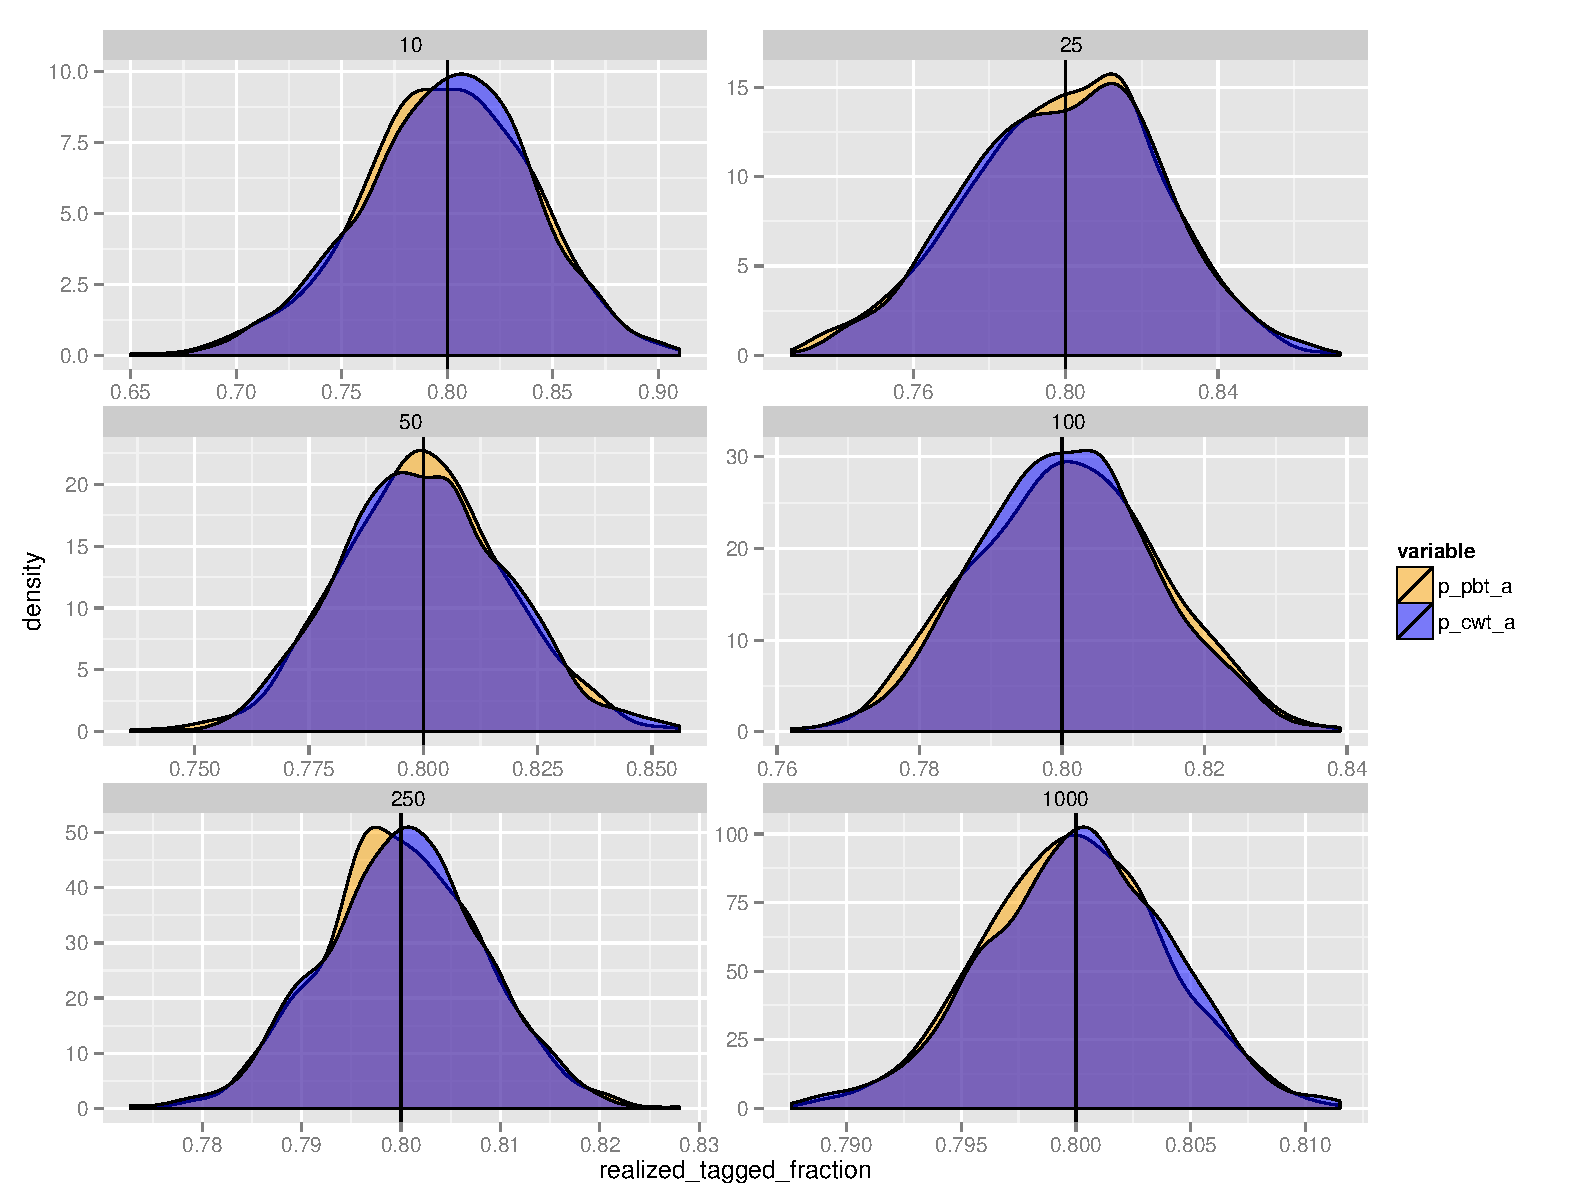
\includegraphics[width = .48\textwidth]{images/tag_fracts_80_WrightFisher.pdf}
	}~~~~~
	\subfigure[$G = \lfloor0.96S\rfloor$]{
		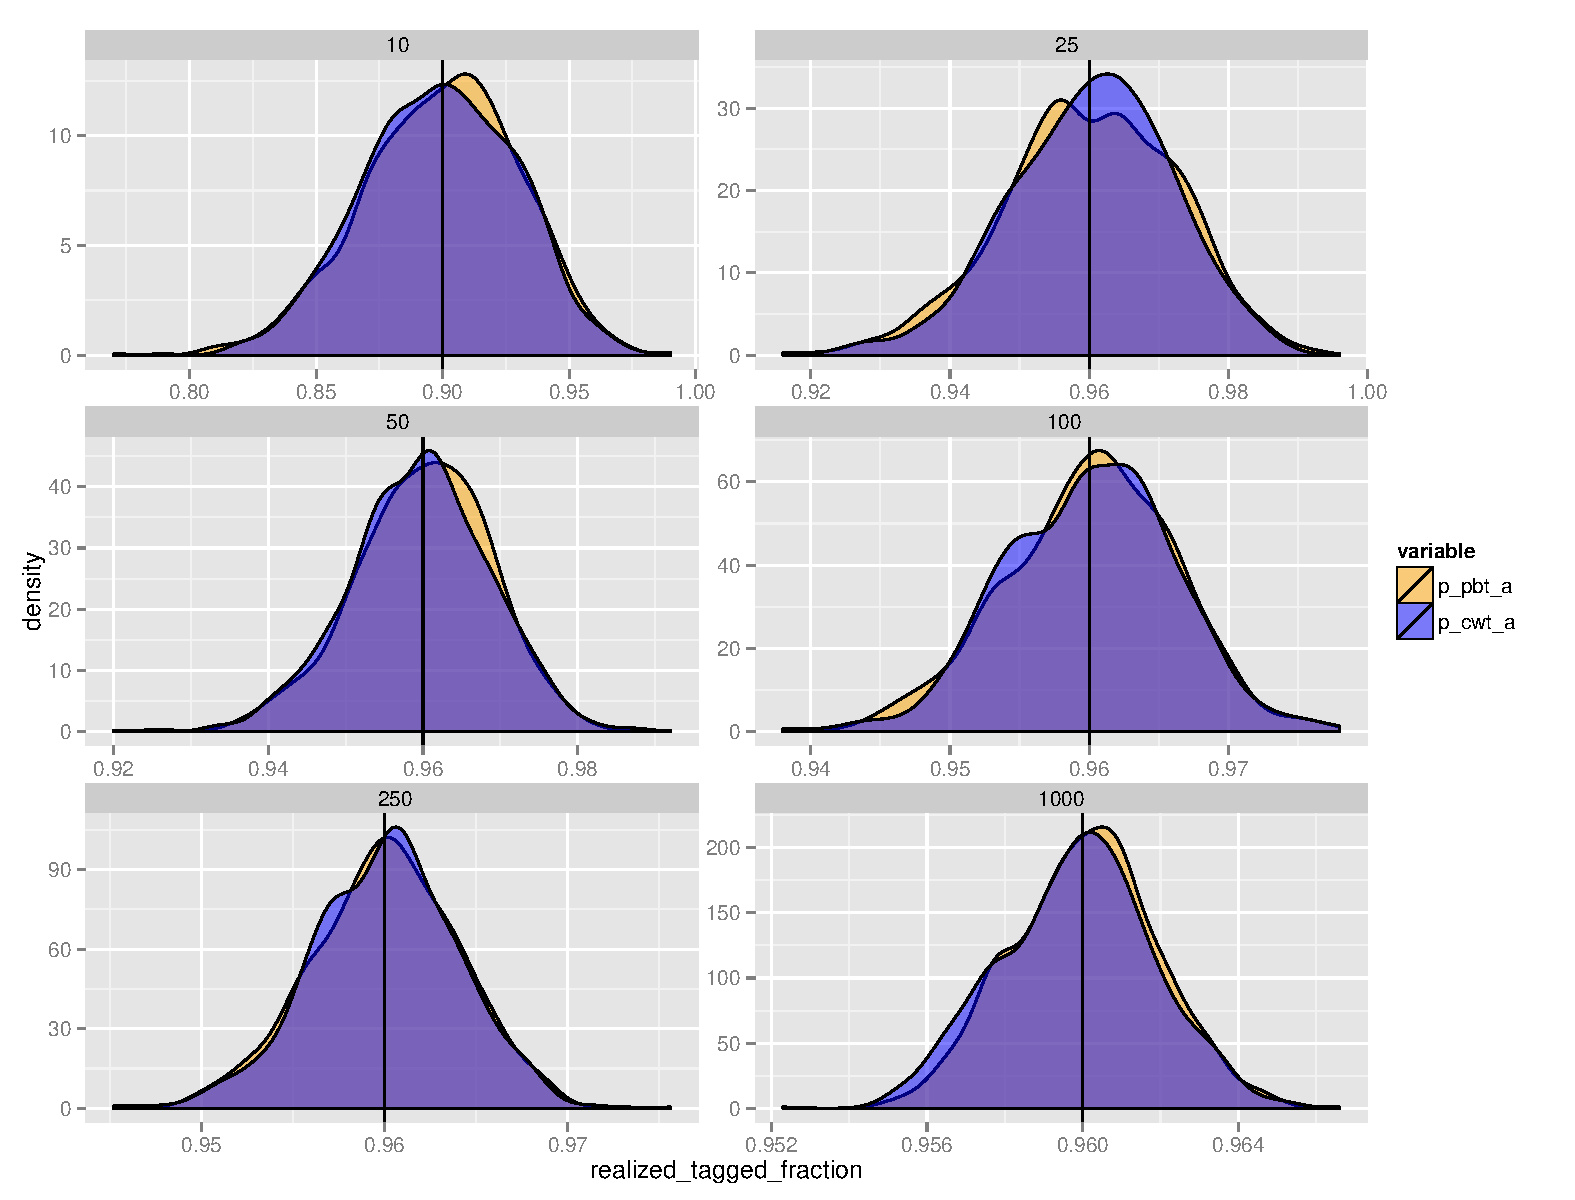
\includegraphics[width = .48\textwidth]{images/tag_fracts_96_WrightFisher.pdf}
	}
}
\caption{Density estimates of the distribution of realized tagging fractions under PBT (orange) and CWT (blue) scenarios
in Simulation~1 with $\frac{N_b}{2S} = 1$ (i.e., Wright-Fisher variance in reproductive success). Number of successfully tagged families
equal to $G = \lfloor0.80S\rfloor$ in ({em a}) and $G = \lfloor0.96S\rfloor$ in ({\em b}).  Numbers
atop each panel give $S$, the number of families contributing to the release group. The black vertical line
gives the true fraction of families successfully genotyped or tagged at release by CWTs. Note that
scales differ between panels.}
\label{fig:wf80}
\end{sidewaysfigure}




%%% Second histogram 2-subfigures (Ne/N = 0.5)
\begin{sidewaysfigure}
\centering
\mbox{
	\subfigure[$G = \lfloor0.80S\rfloor$]{
		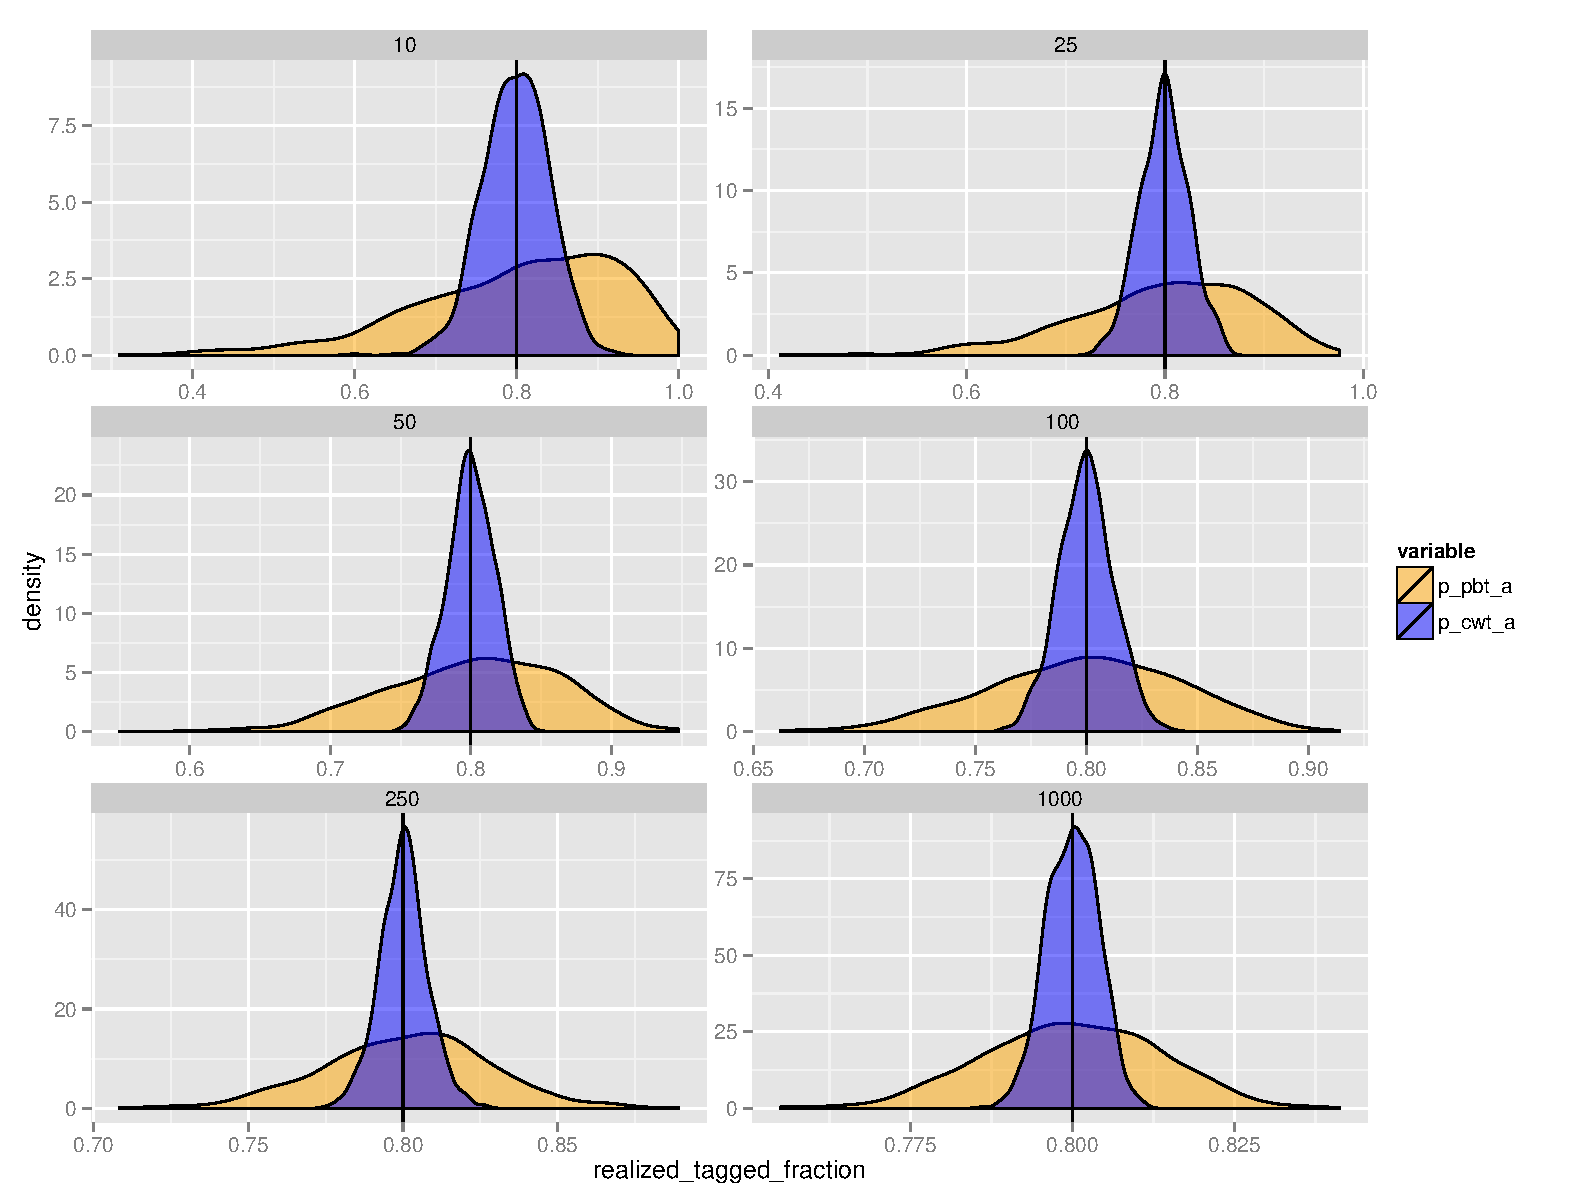
\includegraphics[width = .48\textwidth]{images/tag_fracts_80_Ne50.pdf}
	}~~~~~
	\subfigure[$G = \lfloor0.96S\rfloor$]{
		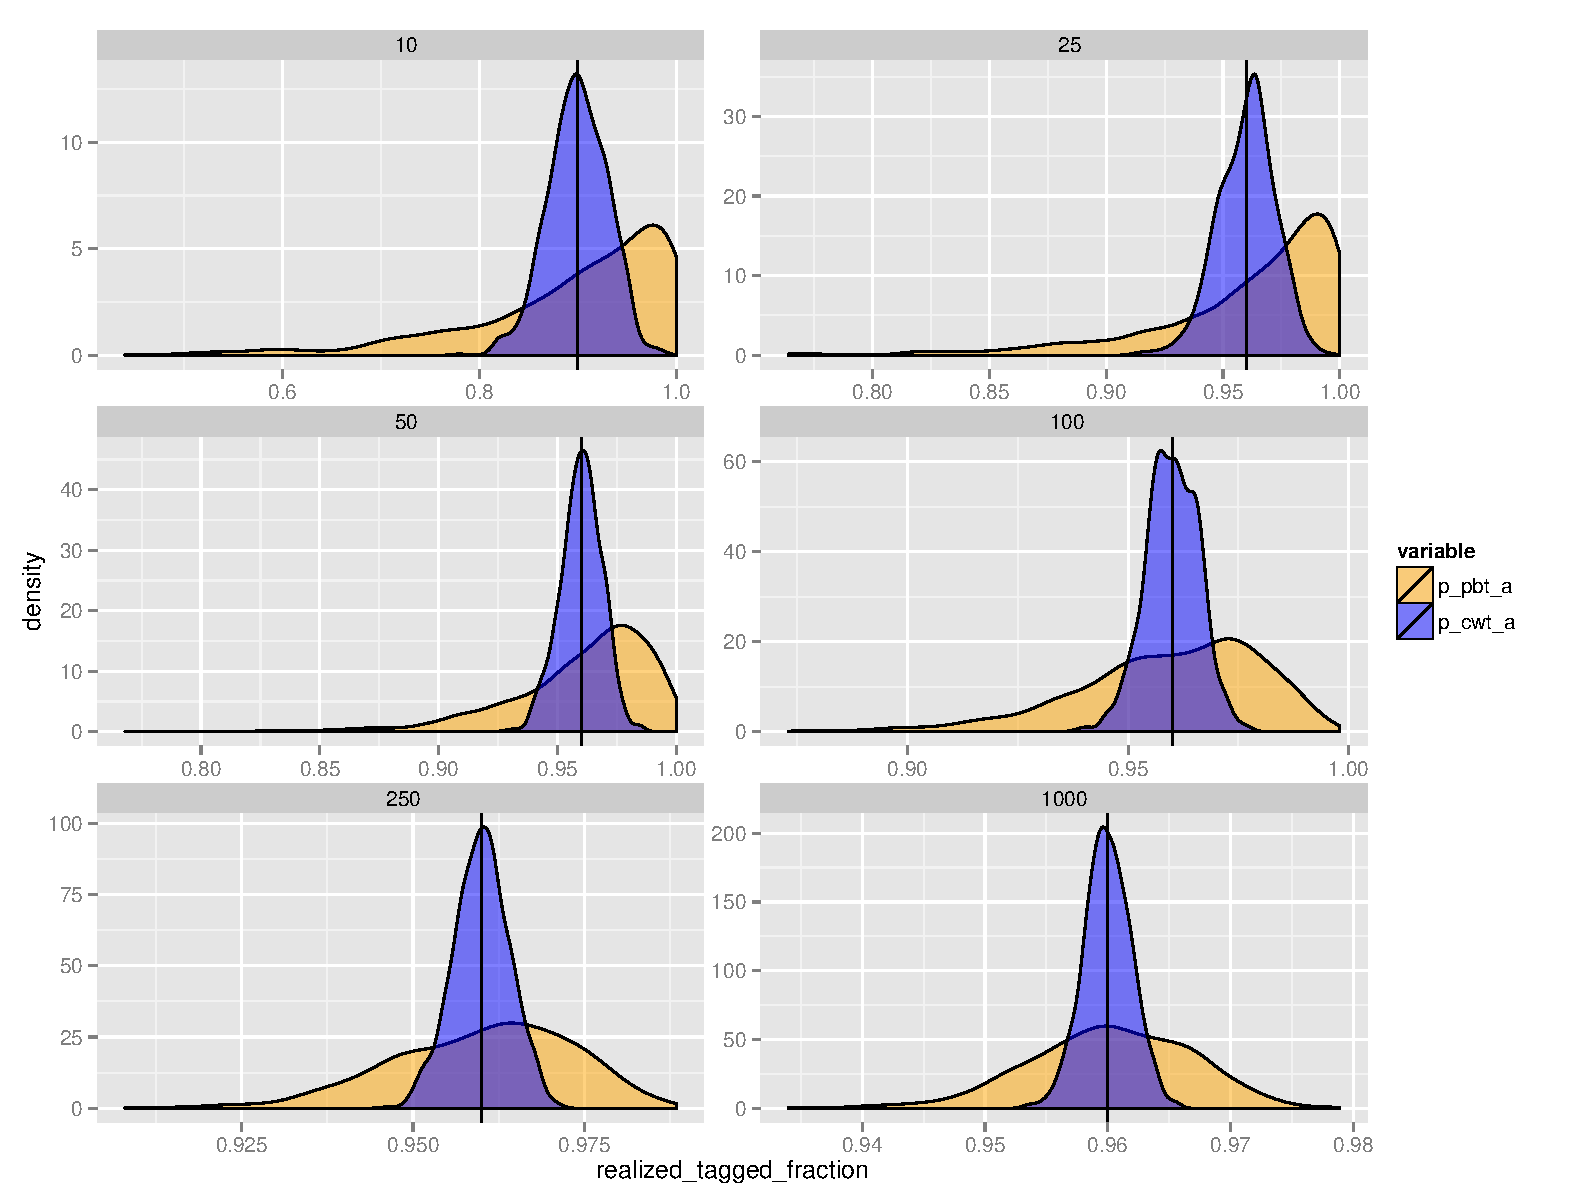
\includegraphics[width = .48\textwidth]{images/tag_fracts_96_Ne50.pdf}
	}
}
\caption{Density estimates of the distribution of realized tagging fractions under PBT (orange) and CWT (blue) scenarios
in Simulation~1 with $\frac{N_b}{2S} = 0.5$. Number of successfully tagged families
equal to $G = \lfloor0.80S\rfloor$ in ({em a}) and $G = \lfloor0.96S\rfloor$ in ({\em b}).  Numbers
atop each panel give $S$, the number of families contributing to the release group. The black vertical line
gives the true fraction of families successfully genotyped or tagged at release by CWTs. Note that
scales differ between panels.}
\label{fig:Ne50}
\end{sidewaysfigure}




These simulations show that, if salmon populations reproduced in a Wright-Fisher fashion
(\ie Poisson distribution of family sizes), then the variation in
realized tagging rates for PBT would be commensurate with those for CWTs.  However, salmon populations
typically exhibit variance in reproductive success beyond that expected in a Wright-Fisher population, with
$N_b/(2S)$ ratios in  Oregon coho hatcheries reported to be between 0.76 and 0.84  \citet{Moyeretal2007}. 
 In such cases with overdispersed variance in reproductive success,
for release groups arising from few families ($<50$ families, for example),
there is an appreciable increase in the variance of the realized tagged fraction of adults using PBT when
not all of the parents were successfully genotyped.  However,
the consequence of this for different applications needs to be assessed. Accordingly a second set of simulations
was conducted in which the goal was to assess the effect on expanded numbers of fish. 

\section{Simulation~2. Implications for Expanded Estimates}

Simulation~1 assesses the variance in the realized tagging rate that corresponds to a situation in which
the goal is to PBT-tag 100\% of a release group, but due to genotyping failures, some fraction
of families are not tagged.  The comparison between CWTs and PBT in those simulations
make it clear that for a given total tagging rate of a release group, PBT will always have a higher
variance in the realized adult tagging rate than CWTs.  However, CWTs are not always applied to
100\% of a release group.  Rather, CWTs are often applied to only a fraction of a release group, and then
only a fraction of a fishery or the escapement might be sampled for tags.
Recoveries of tags (from a fishery, for example) are expanded, by muliplying by the reciprocal of the
catch sampling rate, into a representation of the number of tagged fish from the release group present in the
total catch from the fishery.  That number might be expanded further, multiplying by the reciprocal of the
tagging rate, to give an estimate of the total number of fish from the release group (whether
tagged or not) in the catch.  Therefore, to understand the consequences of tagging rate
variation on the uncertainty of release-group-specific estimates of total fish caught in a fishery, it is necessary to understand the 
sampling context in which tagged fish are recovered. Simulation~2 attempts to provide that context.  

\subsection{Simulating expanded catch estimates}

In Simulation~2, under the PBT scenario, each release group is, as before, descended from $S$ families, of which $G$ are successfully tagged.  However, a fraction
$c$ of the release group is marked in such a way as to be subject to sampling.  In the simulated fishery, there are $N_C$ fish from
the release group in the total catch, but only a fraction $v$ of the total catch is sampled for marks.  Accordingly, the expected fraction of fish 
from the release group expected to yield tag recoveries is $\frac{cvG}{S}$.   If $n_\mathrm{pbt}$ tags were recovered,
the expanded estimate of $N_C$, the
total number of fish from the release group in the catch, would be $\hat{N}_\mathrm{pbt} = \frac{n_\mathrm{pbt}S}{cvG}$.
The PBT scenario is compared against a CWT scenario in which a fraction $c$ of the release group is marked, and 100\% of those marked fish
carry CWTs (i.e., assume for simplicity that the rate of tag shedding is 0).  $N_C$ fish from the release group appear in the total catch,
and a fraction $v$ of the fishery is sampled for marks, yielding $n_\mathrm{cwt}$ recoveries and an expanded estimate of
$\hat{N}_\mathrm{cwt} = \frac{n_\mathrm{cwt}}{cv}$ fish from the release group in the total catch.  


It is worth mentioning that while we refer to fish as being ``marked'' these simulations apply equally well to both visually
and electronically sampled fisheries.  In the visual case, a fraction $c$ of the fish are ad-clipped and all of those are
carry CWTs (in the CWT scenario), or a fraction $G/S$ are expected to be tagged with PBT (in the PBT scenario).  
In the electronic case, the PBT scenario is 
equivelent to a random fraction $c$ of the fish in the release group receiving AWTs that will trigger electronic detectors
and lead to genotyping of the fish, while the CWT scenario is equivalent to a fraction $c$ of the release group
carrying CWTs.   


The effect of $c$ and $v$ on the estimates always acts through their product, and, in Simulation~2 we can
simply model their product $m = cv$---the fraction of the release group in the catch that is tagged and subject to sampling.
For PBT simulation replicates we first simulate $\tilde{p}_\mathrm{pbt}$ as in Simulation~1, and then we
simulate the number of PBT-tagged fish recoveries as $n_\mathrm{pbt}\sim\mathrm{Binomial}(N_C, m \tilde{p}_\mathrm{pbt})$, from which 
we compute and record $\hat{N}_\mathrm{pbt} = \frac{n_\mathrm{pbt}S}{mG}$.  For the CWT simulation replicates, we simulate the number of sampled
and tagged fish in the total catch as $n_\mathrm{cwt} \sim \mathrm{Binomial}(N_C, m)$, and from that compute
$\hat{N}_\mathrm{cwt} = \frac{n_\mathrm{cwt}}{m}$.
 
 
\subsection{Simulation 2 settings} 

500 replicate simulations were performed for every combination of the following set of values:
\begin{itemize}
\item $S \in \{10, 20, 30, 50, 100, 200, 400, 1000\}$
\item $N_C = N_A = 50$
\item $G \in \{\lfloor a S\rfloor\}$ where $a \in \{0.80, 0.82, \ldots, 0.98, 1.00\}$, and with $p_\mathrm{cwt}$ set to the same
value as $\lfloor a S\rfloor$ in each case.
\item $\mu = 3000$, $r = 30$, and $\alpha \in \{0.3, 0.5, 1.0, 2, 10\}$, as well as an additional scenario corresponding to
Wright-Fisher reproduction. 
\item $m \in \{0.125, 0.25, 0.5, 0.75, 1.0\}$
\end{itemize}


Each of the different scenarios of family size variance produced a different ratio of $N_b/(2S)$ covering a broad range:
$(0.25, 0.34, 0.50, 0.66, 0.88, 1.00)$, we summarize the results in terms of these $N_b/(2S)$ ratios
rather than in terms of $\alpha$, $\mu$, and $r$.



%Figure~\ref{fig:all_sds} summarizes the standard deviation of the realized PBT and CWT tagging rates across all the scenarios.
%\begin{sidewaysfigure}
%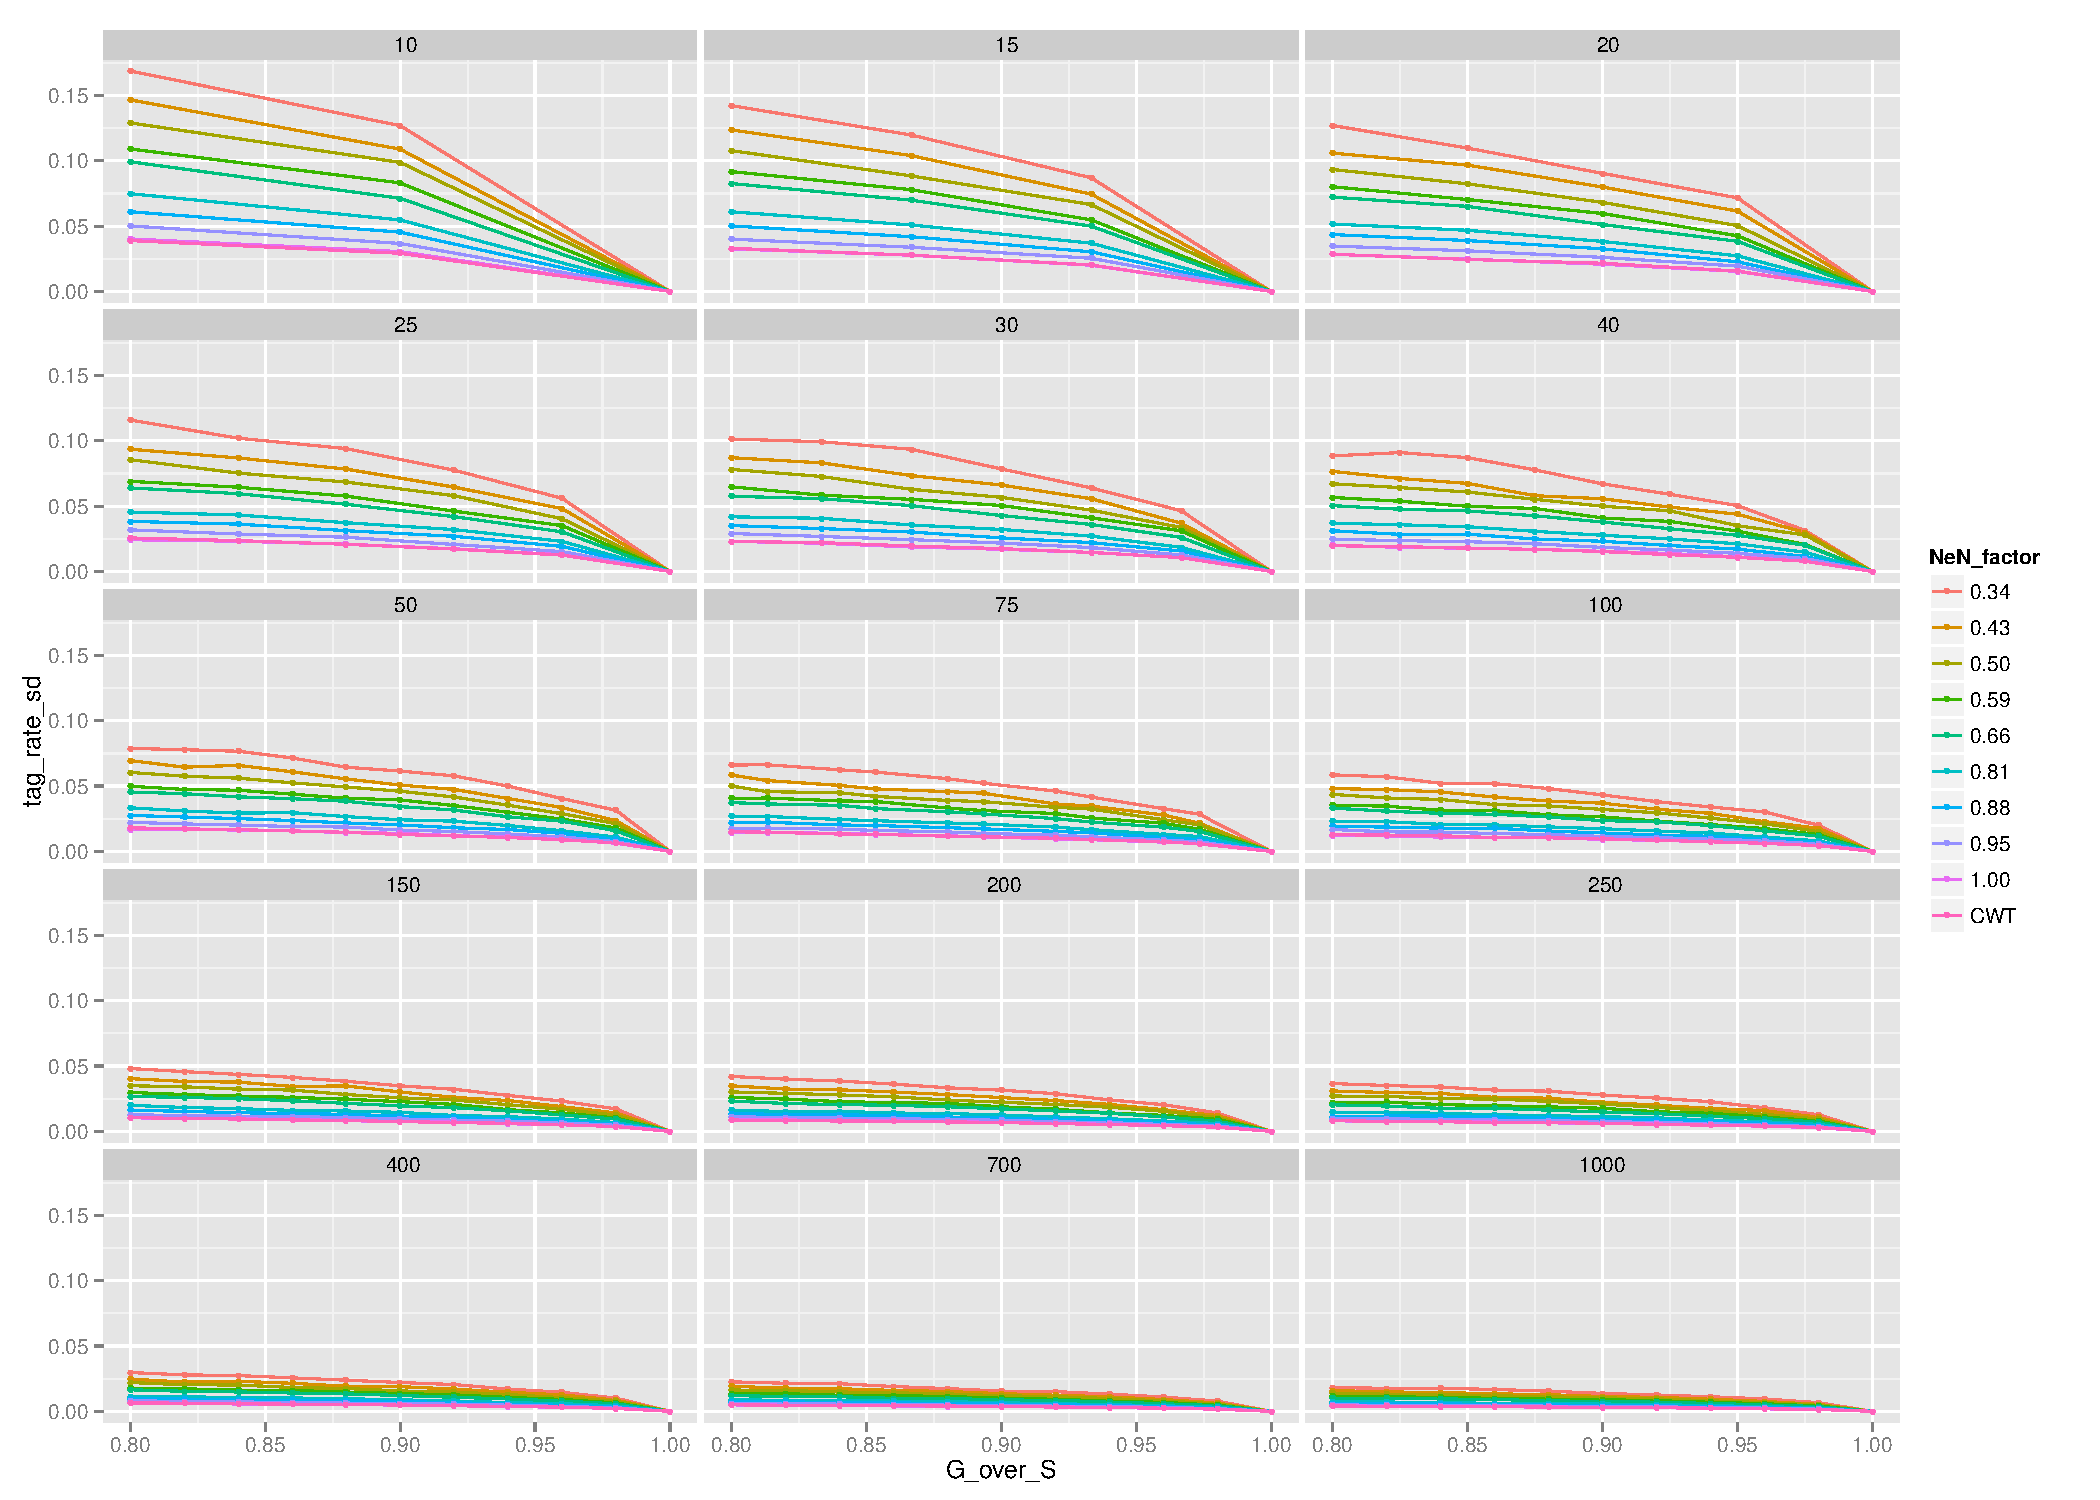
\includegraphics[width = .93\textwidth]{./images/tag_rate_standard_devs.pdf}
%\caption{The standard deviation of the realized tagging rate $\tilde{p}_\mathrm{pbt}$ and $\tilde{p}_\mathrm{cwt}$.  $x$ axis shows the
%expected tagged fraction $\lfloor G/S \rfloor$ in each simulation, $y$-axis gives the standard deviation over 1000 simulation replicates
%for each point.  Colors denote different $N_b/(2S)$ ratios for PBT (or they denote CWT tagging in the bottom line in every panel).  Different
%panels correspond to different numbers of $S$, as denote on the top of each panel.
%\label{fig:all_sds}}
%\end{sidewaysfigure}
%It is clear that the variance of the realized PBT tagging rate is always higher than that of the CWT tagging rate, except in the case where
%$N_b/(2S) = 1.0$, in which case the two are identical.  Standard deviation of $\tilde{p}_\mathrm{pbt}$ increases as $N_b/(2S)$ decreases and
%as $S$ decreases.  


Figures~\ref{fig:horn0.125}--\ref{fig:horn1.0} display the standard deviation of the estimators
$\hat{N}_\mathrm{pbt}$ and $\hat{N}_\mathrm{cwt}$.  Several clear trends emerge.  First, when 
$m\leq 0.25$, the effect of the extra  variance in the PBT tagging rate has a relatively small
effect on the variance of $\hat{N}_\mathrm{pbt}$, even when$S$ is as small as 10.  When $m\geq 0.5$
the effect of the PBT tag rate variance is more noticeable, especially at values of $S$ less than
30.  If $m=1.0$, then the PBT tag rate variance is relatively important at all values of
$S$.  This is not too surprising, since there is no variance in $\hat{N}_\mathrm{cwt}$ in that
case.  However, it is also clear that the extra variance incurred from PBT is not very large
for family tagging fractions greater than 0.096 or 0.98.  It must also be kept in mind that
CWTs will seldom achieve a 100\% tag rate, since there is usually some measurable degree of
tag shedding.   As expected, the influence of PBT tag rate variance increases when $N_b/(2S)$
decreases.

Overall, the results indicate that the additional variance in expanded estimates,
$\hat{N}_\mathrm{pbt}$ due to the variance in the PBT tagging rate is somewhat unremarkable 
when the fraction of tagged families is greater than 98\%, regardless of $S$.  If 
$G/(2S)$ is less then 0.98, however, then the additional variance only becomes truly 
noteworthy when $S<50$, $N_b/(2S) < 0.7$ and $m > 0.5$.

Thus, the relative importance of PBT tagging rate variance to the overall uncertainty of 
expanded estimates depends on the the range of values of those parameters that are
likely to be encountered in practice.  Such values are explored in the following section.

% m = 0.125
\begin{sidewaysfigure}
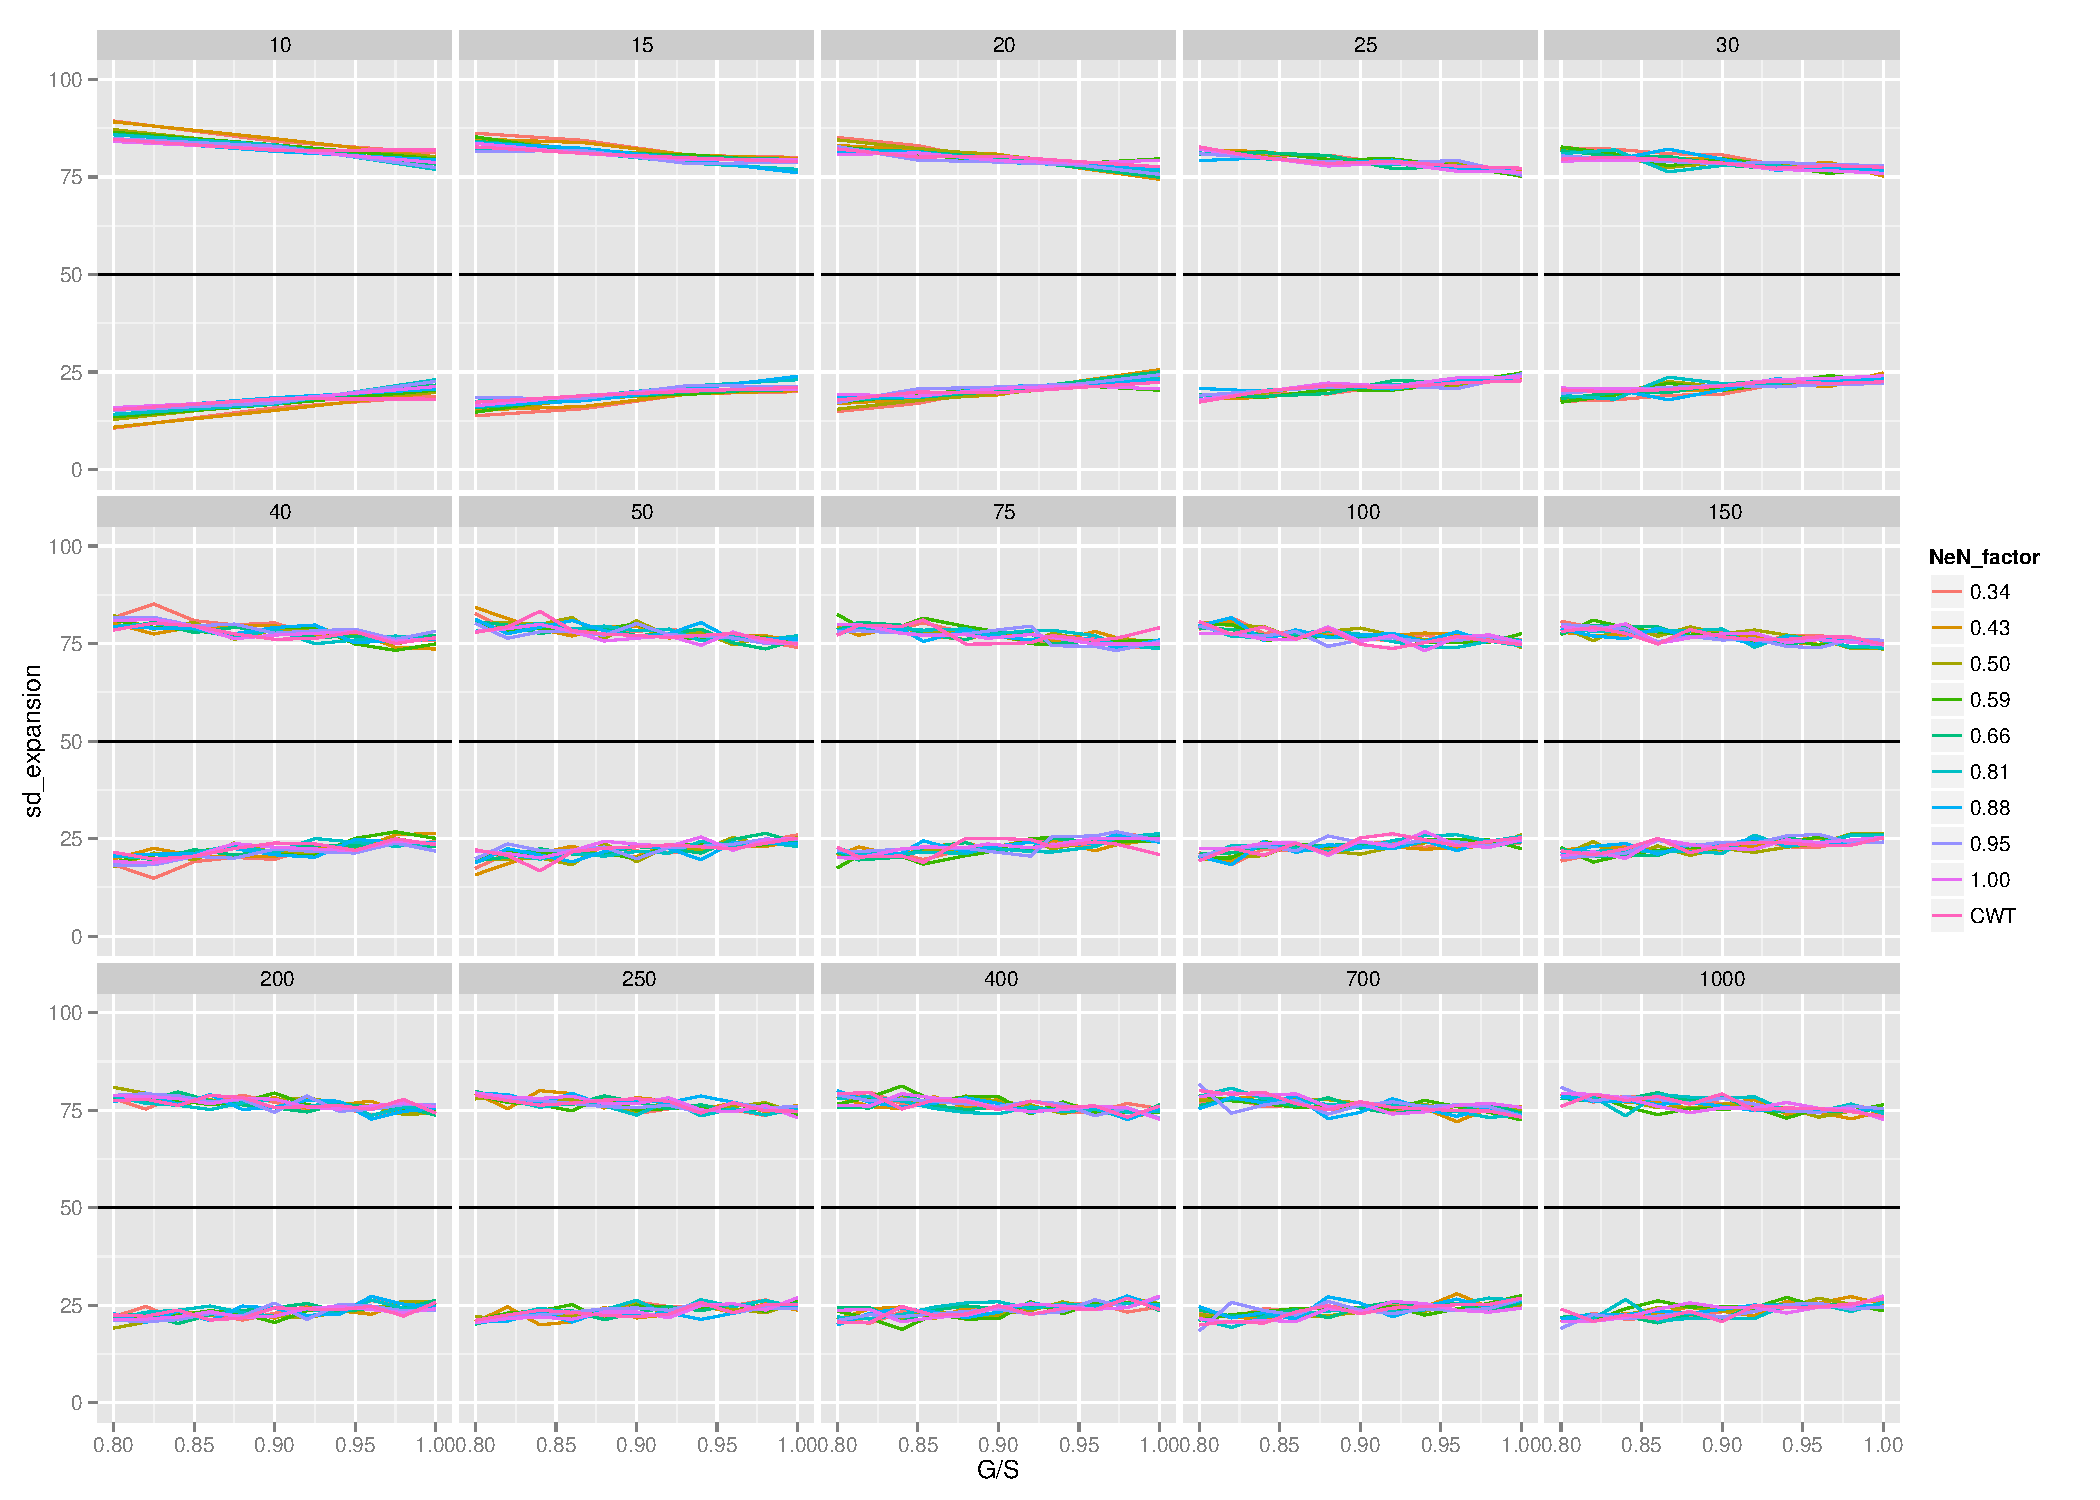
\includegraphics[width = .93\textwidth]{./images/sd_line_horns_m_0_25.pdf}
\caption{The uncertainty around expanded estimates using PBT or CWTs when $m = 0.25$.  $x$ axis shows the
expected tagged fraction $\lfloor G/S \rfloor$ in each simulation. Upon the $y$-axis is the number of fish from the
release group in the fishery (shown as the black horizontal line) and the mean estimate of that number from each different set of 
conditions plus or minus 2 standard deviations.  Thus, the vertical spread between lines of the same colour gives a representation
of the uncertainty in the estimate of the expanded number of fish. Colors denote different $N_b/(2S)$ ratios for PBT, or denote
the CWT estimate.  Different
panels correspond to different numbers of $S$, as denoted on the top of each panel.
\label{fig:horn0.125}}
\end{sidewaysfigure}



% m = 0.25
\begin{sidewaysfigure}
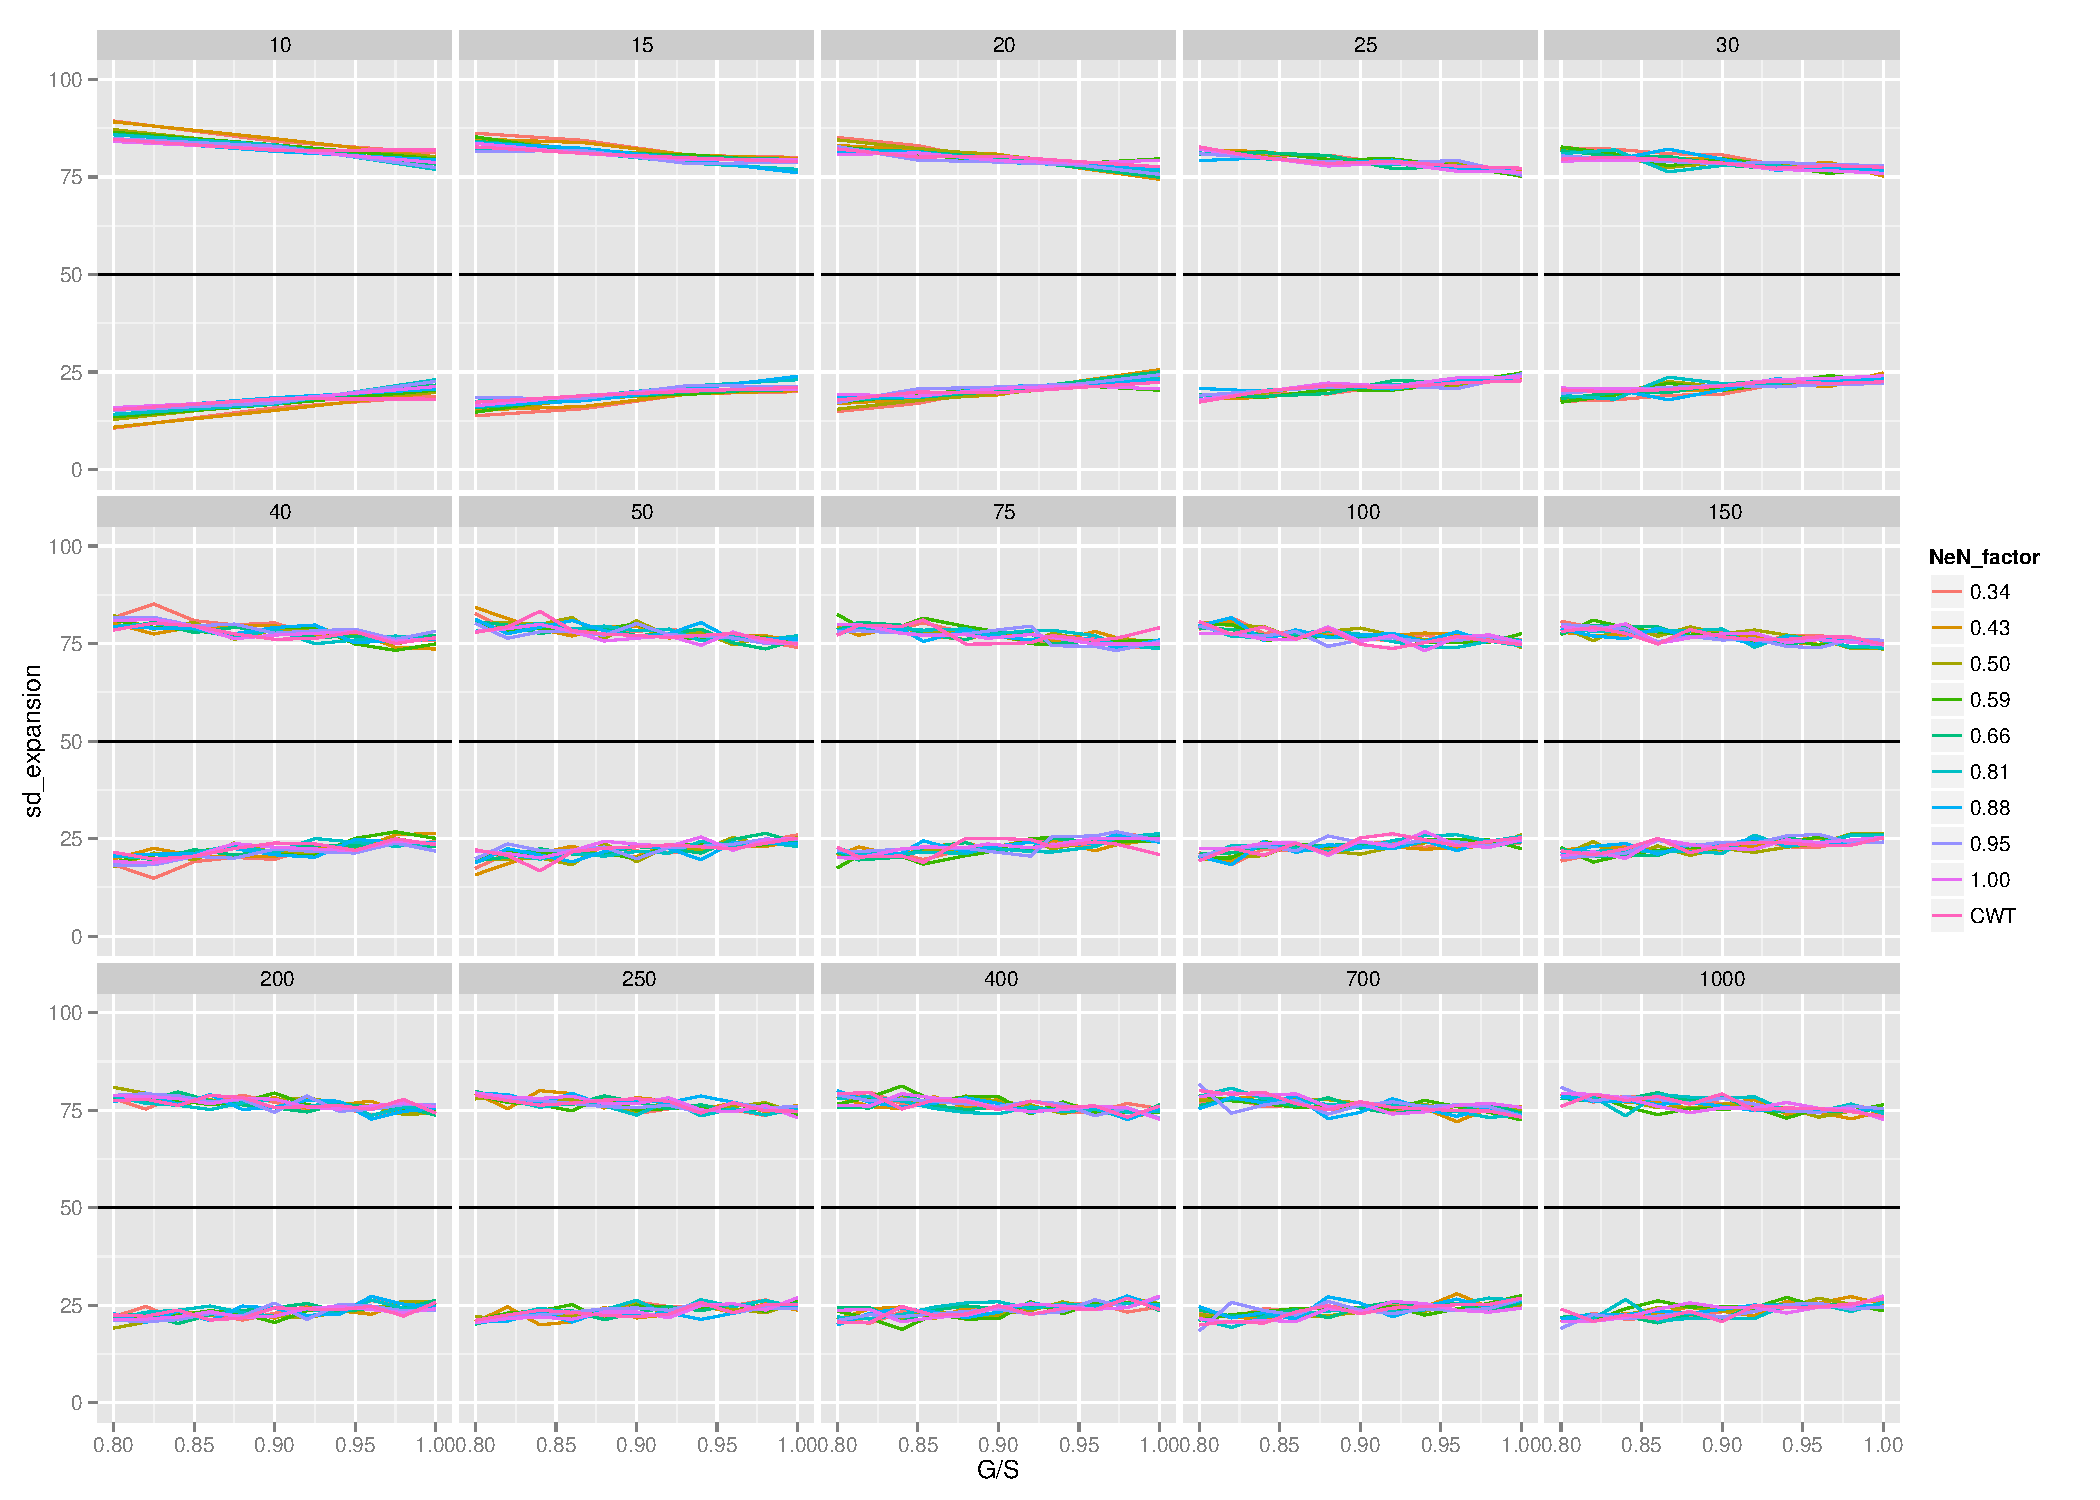
\includegraphics[width = .93\textwidth]{./images/sd_line_horns_m_0_25.pdf}
\caption{The uncertainty around expanded estimates using PBT or CWTs when $m = 0.25$.  $x$ axis shows the
expected tagged fraction $\lfloor G/S \rfloor$ in each simulation. Upon the $y$-axis is the number of fish from the
release group in the fishery (shown as the black horizontal line) and the mean estimate of that number from each different set of 
conditions plus or minus 2 standard deviations.  Thus, the vertical spread between lines of the same colour gives a representation
of the uncertainty in the estimate of the expanded number of fish. Colors denote different $N_b/(2S)$ ratios for PBT, or denote
the CWT estimate.  Different
panels correspond to different numbers of $S$, as denoted on the top of each panel.
\label{fig:horn0.25}}
\end{sidewaysfigure}


% m = 0.5
\begin{sidewaysfigure}
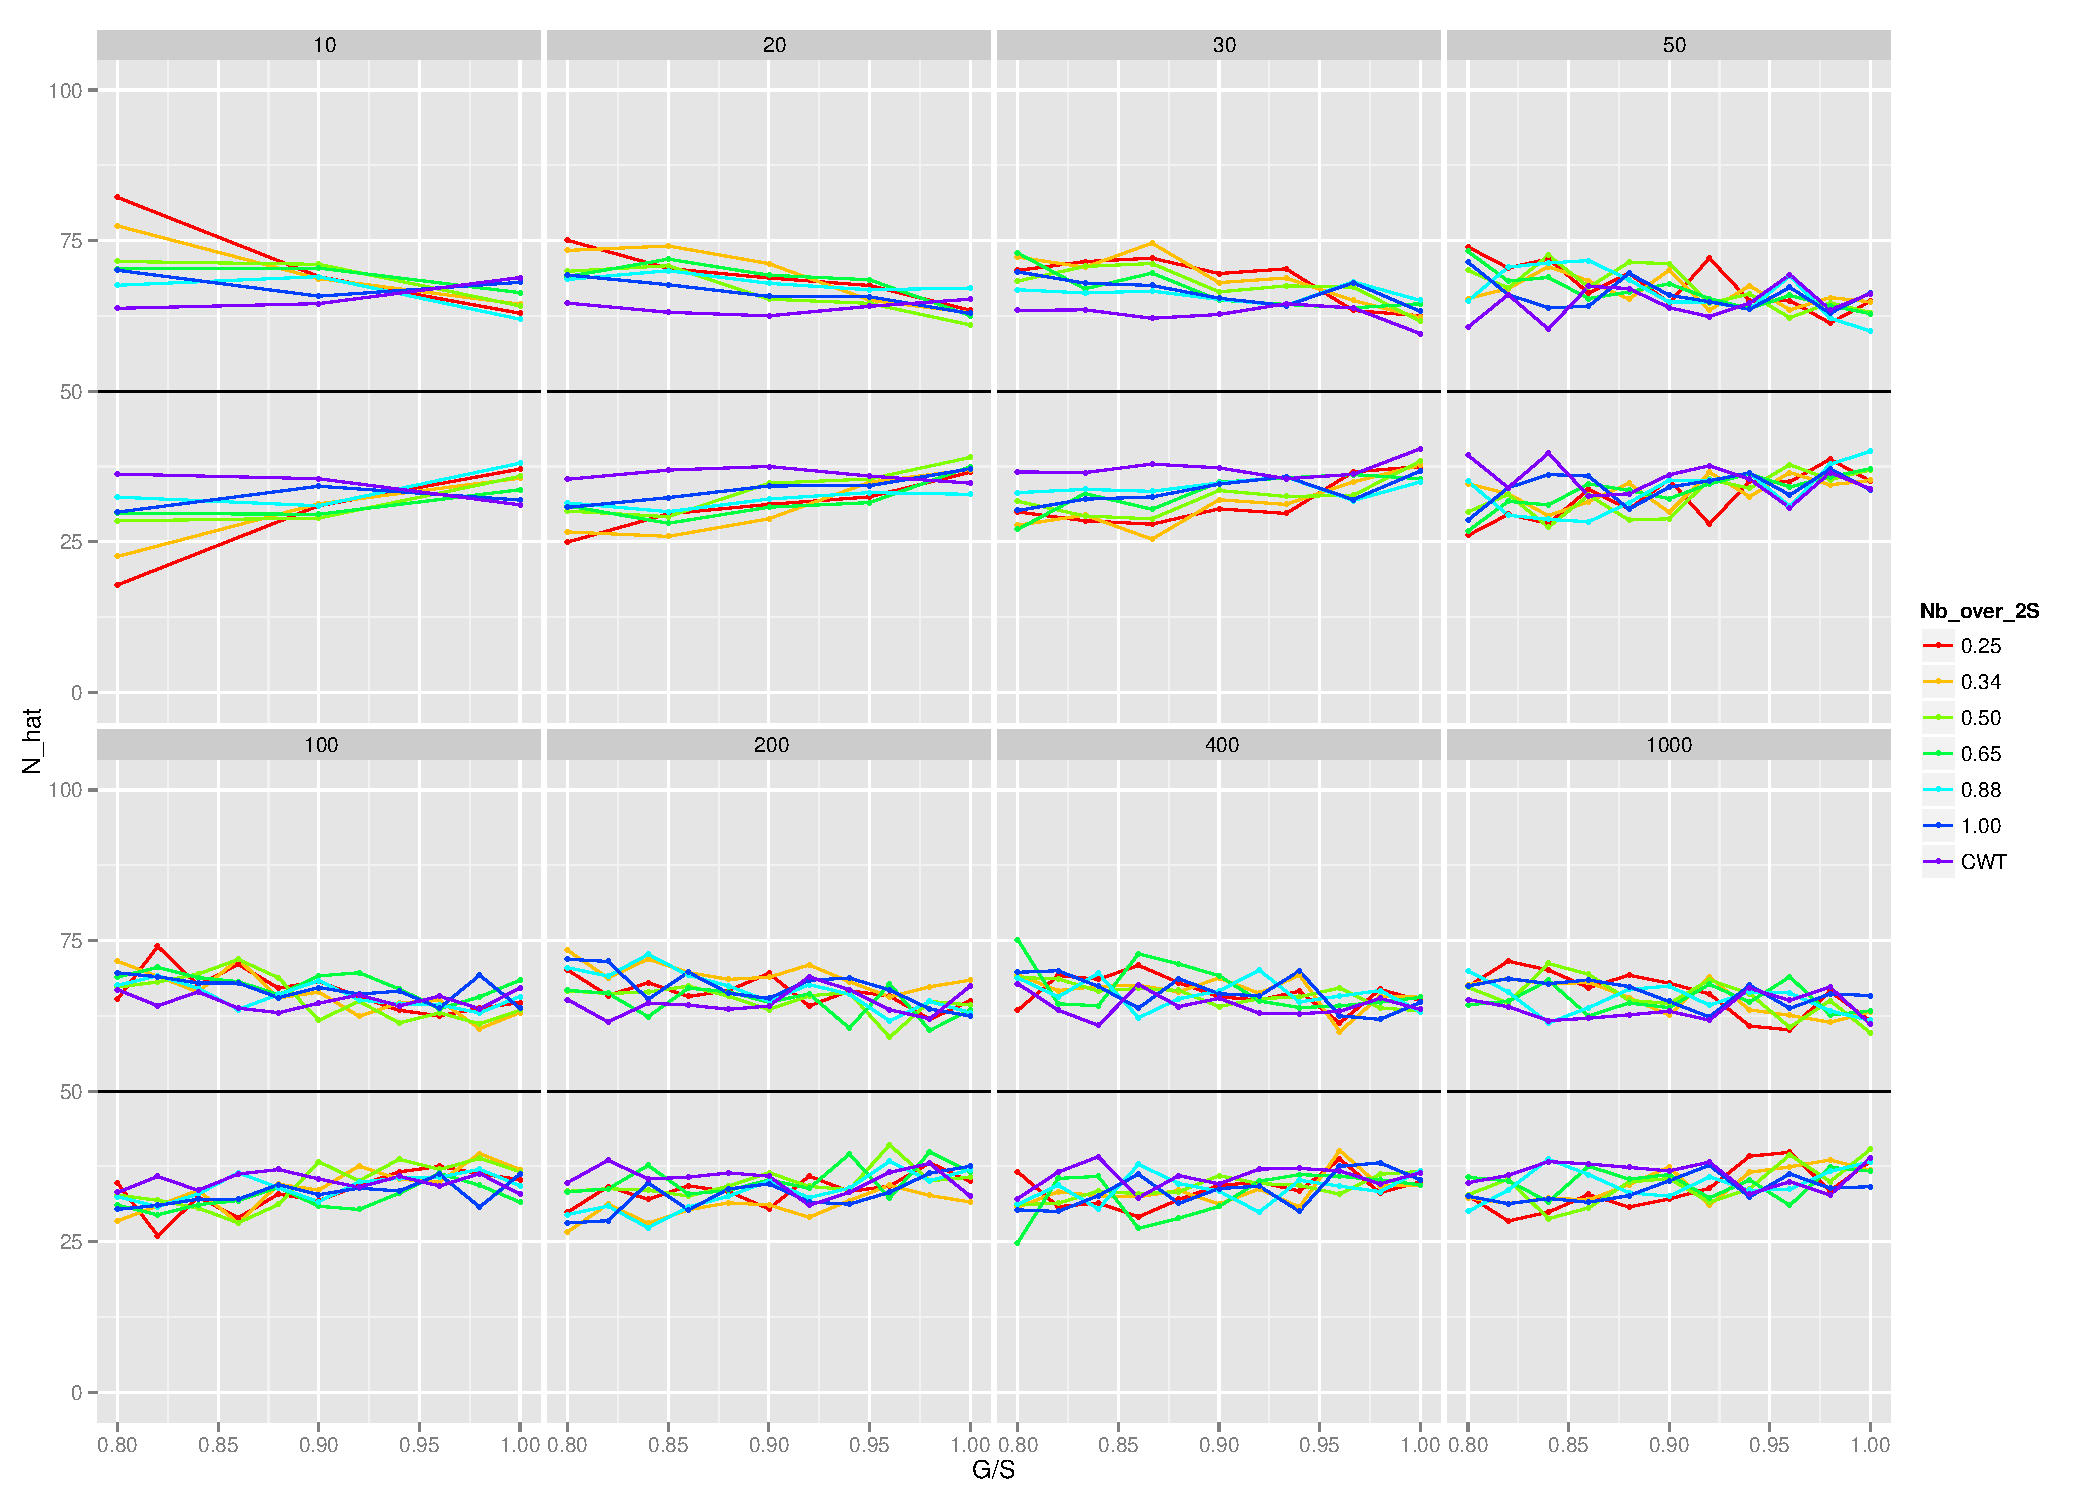
\includegraphics[width = .93\textwidth]{./images/sd_line_horns_m_0_5.pdf}
\caption{The uncertainty around expanded estimates using PBT or CWTs when $m = 0.5$.  $x$ axis shows the
expected tagged fraction $\lfloor G/S \rfloor$ in each simulation. Upon the $y$-axis is the number of fish from the
release group in the fishery (shown as the black horizontal line) and the mean estimate of that number from each different set of 
conditions plus or minus 2 standard deviations.  Thus, the vertical spread between lines of the same colour gives a representation
of the uncertainty in the estimate of the expanded number of fish. Colors denote different $N_b/(2S)$ ratios for PBT, or denote
the CWT estimate.  Different
panels correspond to different numbers of $S$, as denoted on the top of each panel.
\label{fig:horn0.5}}
\end{sidewaysfigure}

% m = 0.75
\begin{sidewaysfigure}
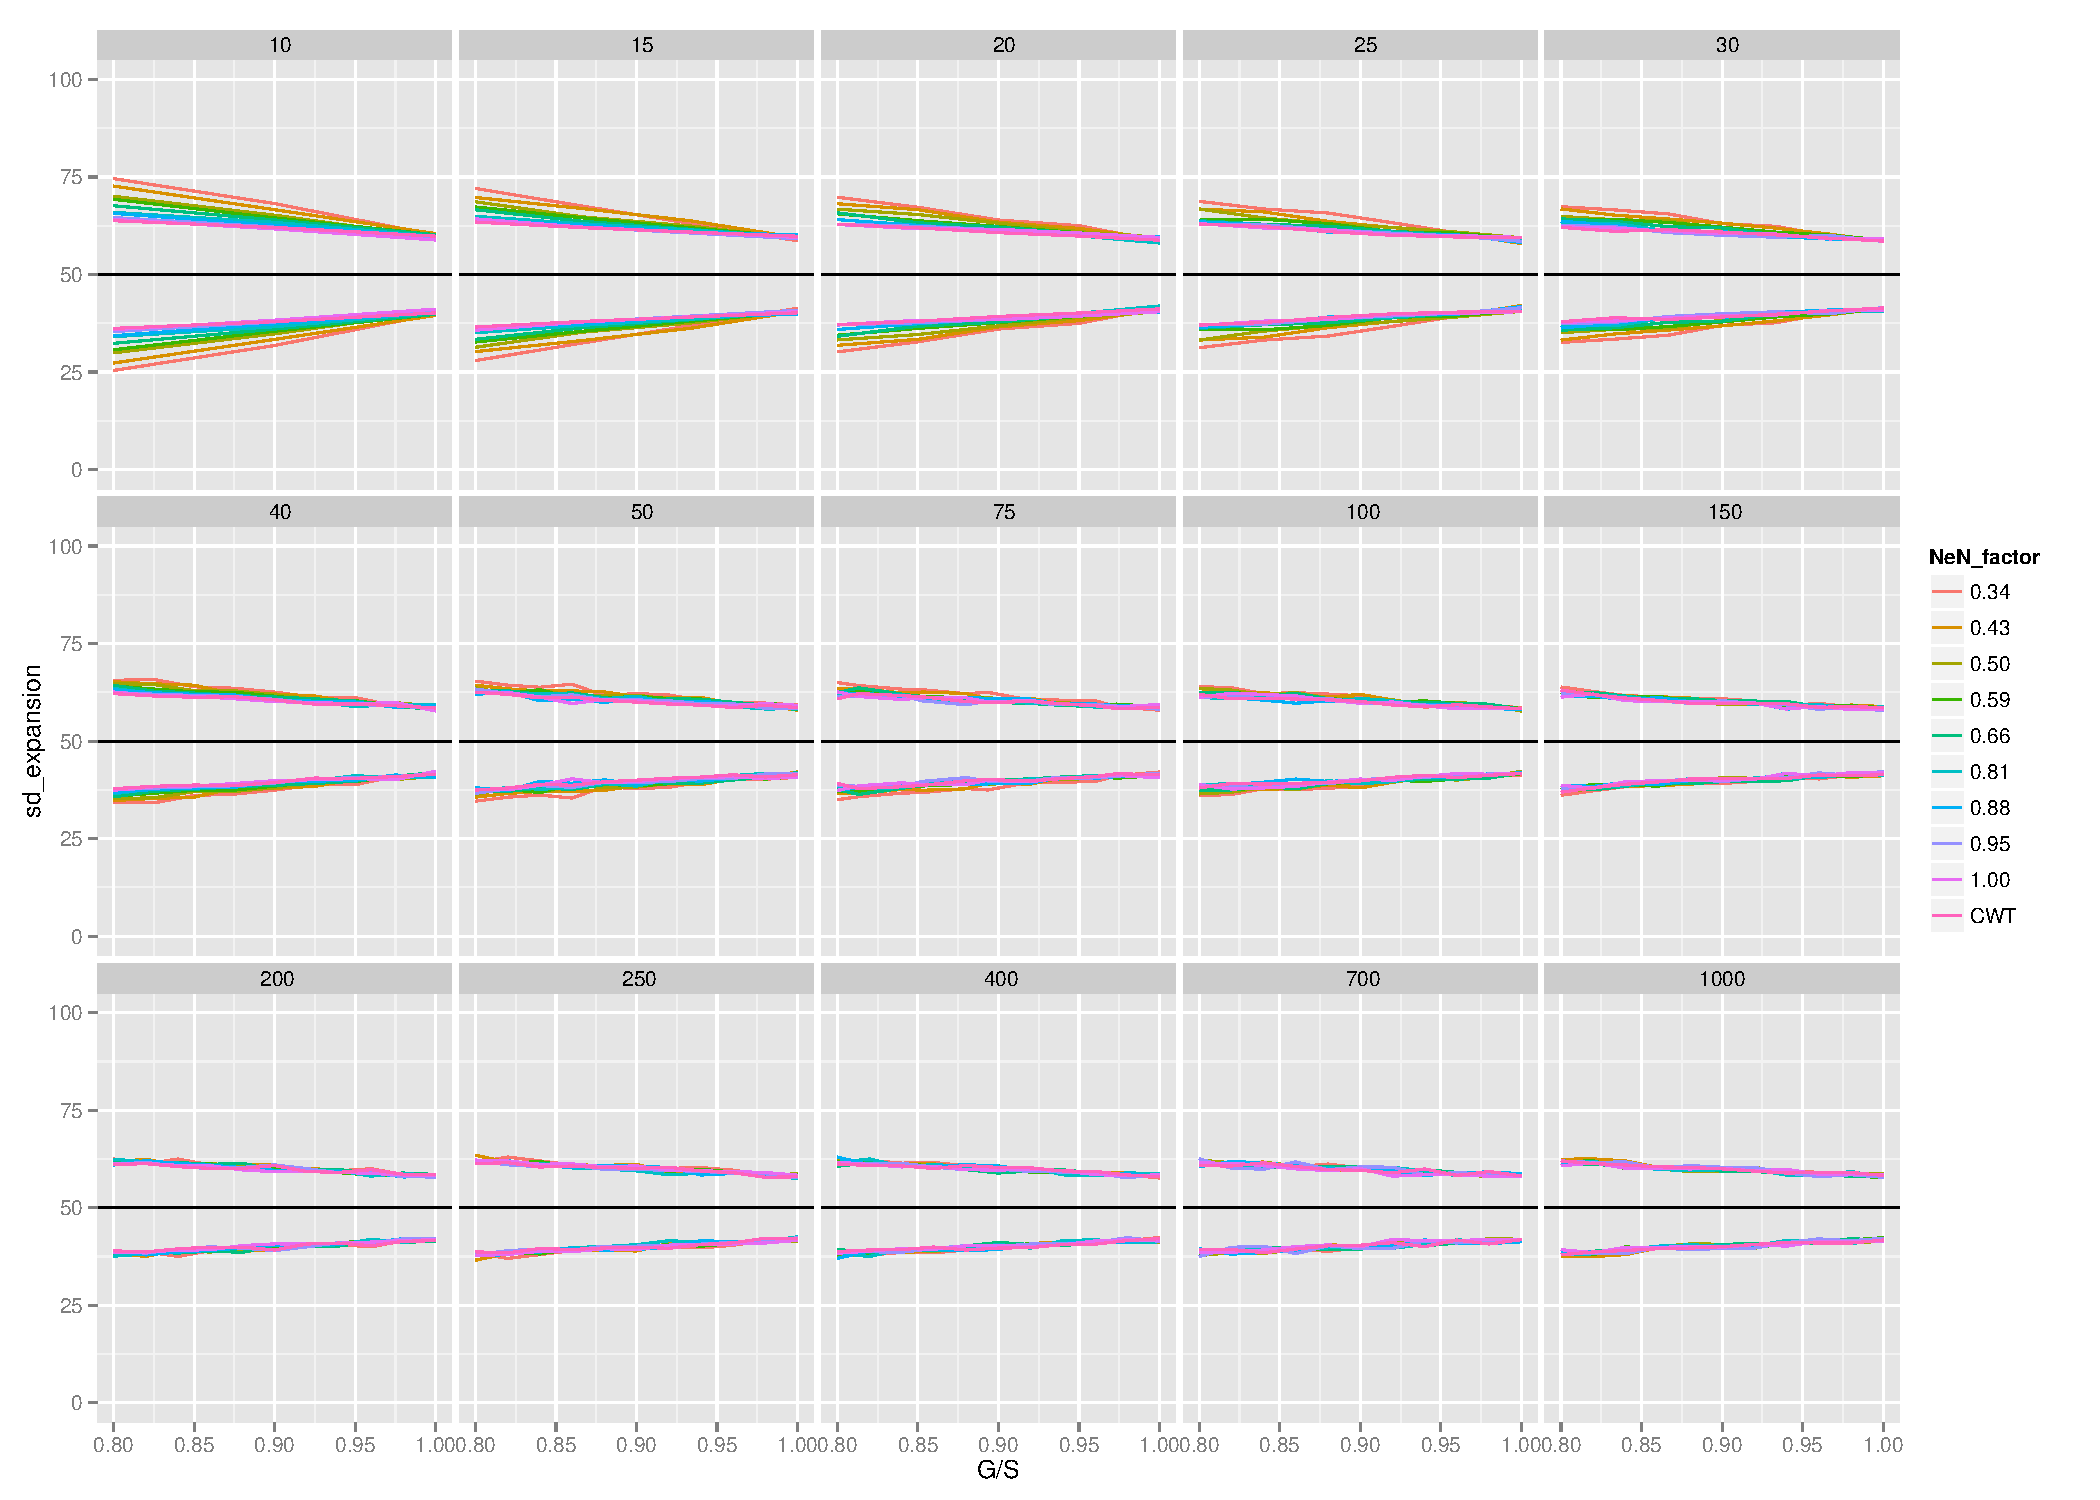
\includegraphics[width = .93\textwidth]{./images/sd_line_horns_m_0_75.pdf}
\caption{The uncertainty around expanded estimates using PBT or CWTs when $m = 0.75$.  $x$ axis shows the
expected tagged fraction $\lfloor G/S \rfloor$ in each simulation. Upon the $y$-axis is the number of fish from the
release group in the fishery (shown as the black horizontal line) and the mean estimate of that number from each different set of 
conditions plus or minus 2 standard deviations.  Thus, the vertical spread between lines of the same colour gives a representation
of the uncertainty in the estimate of the expanded number of fish. Colors denote different $N_b/(2S)$ ratios for PBT, or denote
the CWT estimate.  Different
panels correspond to different numbers of $S$, as denoted on the top of each panel.
\label{fig:horn0.75}}
\end{sidewaysfigure}



% m = 1.00
\begin{sidewaysfigure}
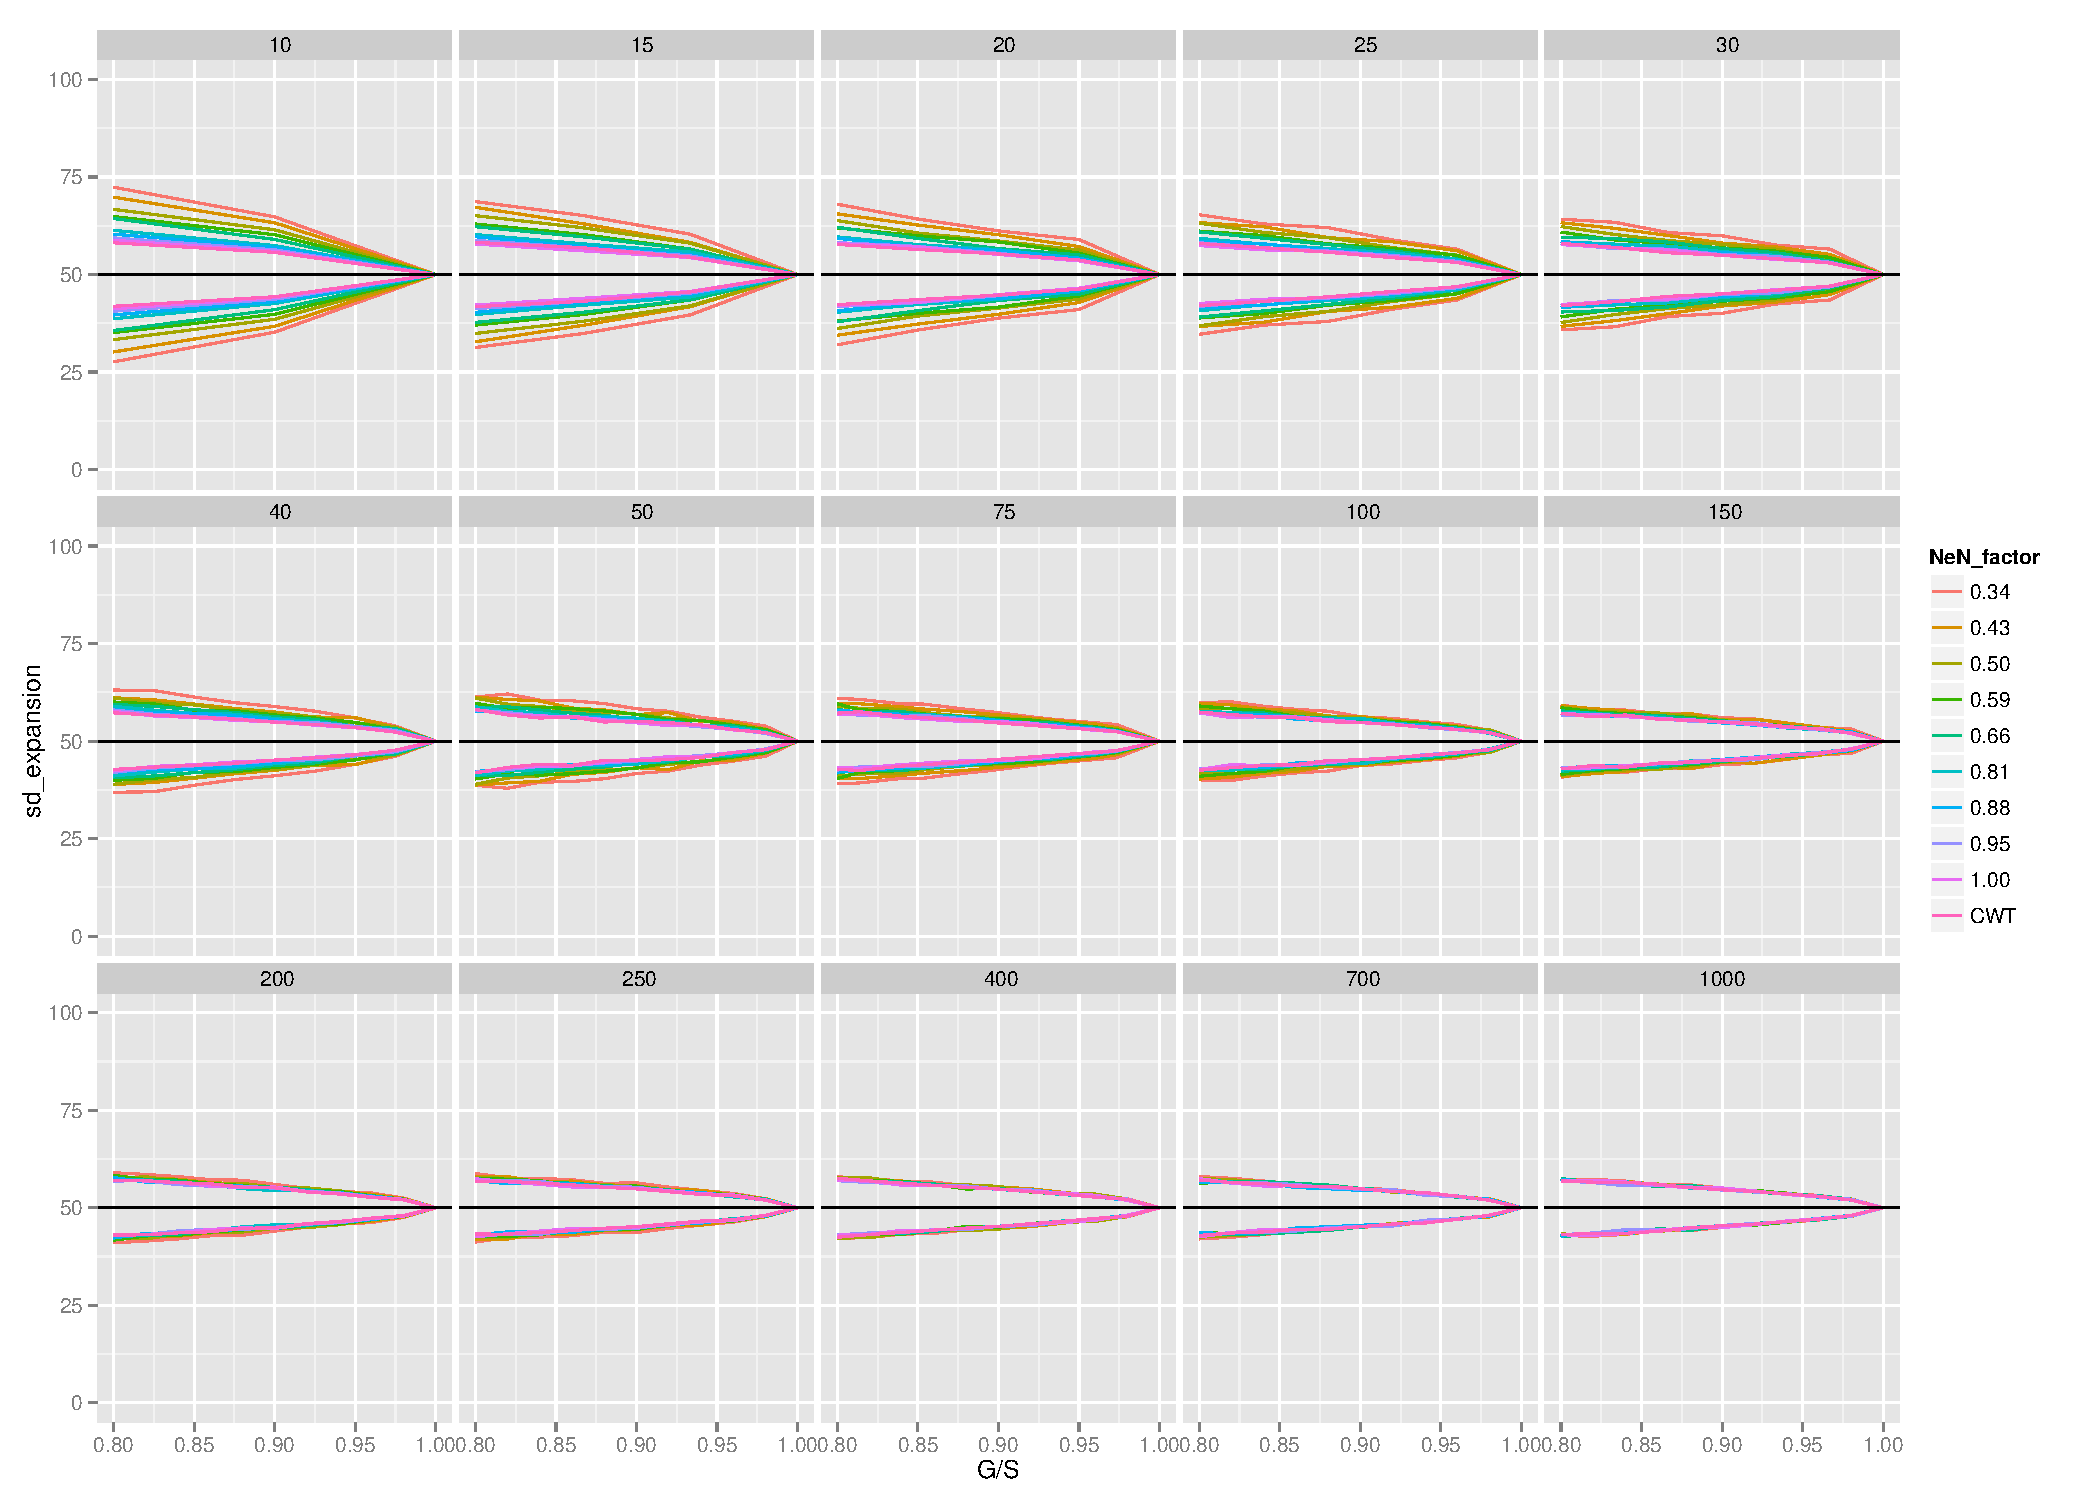
\includegraphics[width = .93\textwidth]{./images/sd_line_horns_m_1.pdf}
\caption{The uncertainty around expanded estimates using PBT or CWTs when $m = 1.00$.  $x$ axis shows the
expected tagged fraction $\lfloor G/S \rfloor$ in each simulation. Upon the $y$-axis is the number of fish from the
release group in the fishery (shown as the black horizontal line) and the mean estimate of that number from each different set of 
conditions plus or minus 2 standard deviations.  Thus, the vertical spread between lines of the same colour gives a representation
of the uncertainty in the estimate of the expanded number of fish. Colors denote different $N_b/(2S)$ ratios for PBT, or denote
the CWT estimate.  Different
panels correspond to different numbers of $S$, as denoted on the top of each panel.
\label{fig:horn1.0}}
\end{sidewaysfigure}



\section{Likely range of parameter values}

\subsection{Effective size of hatchery populations}

Only a few estimates of the ratio of the effective number of breeders to the census number of breeders ($N_b/(2S)$) in salmon
hatcheries are available.  \citet{Moyeretal2007} report estimates of between 0.76 and 0.84 for coho salmon in two different 
Oregon hatcheries.  For Chinook, Mike Ackerman provided the working group with estimates of the number of fish from different
families returning to 5 different
hatcheries in Idaho.  From these data it is possible to estimate a range of $N_b/(2S)$ values from 0.3 to 0.5.


\subsection{Number of families per release group}
The results in Table~\ref{tab:relsummary} gives the size of all CWT-tagged release groups from 2000 forward for
Chinook and coho.  For this analysis, I have assumed that if each release group
were to be tagged via PBT that it arose from spawnings at the hatchery in which the number of male
and female parents is equal and that each Chinook female produces 3,800 offspring that survive to the release stage, and
a coho femal produces 1,800 juveniles survive to release.


%%%%%%%%%%%%%%
\begin{table}
\caption{Summary of tagged chinook releases since brood year 2000 across all agencies.
The No.~releases column gives the number of families that would have been required to
create both the tagged and untagged components of the release group if number of male and female parents were equal and each female
averaged 3,000 smolts surviving to the release stage. The column No.~smolts gives the total number of smolts produced since 2000
in releases requiring number of familes in the range as given in No.~familes.  The column No.~releases gives the number of 
actual release groups in each No.~families category. \label{tab:relsummary}}
\begin{center}
\begin{tabular}{rrrrrr}
\hline\hline
\\
\multicolumn{5}{c}{Chinook}\\
No.~families  &  No.~smolts~released  &  No.~releases  &  \% of all smolts  &  \% of all releases \\ \hline
0--10  &   73,629,227  &  5,138  &  2.40  &  33.72\\
10--25  &  153,197,630  &  3,035  &  4.99  &  19.92\\
25--50  &  248,382,387  &  2,379  &  8.08  &  15.62\\
50--100  &  463,816,013  &  2,177  &  15.10  &  14.29\\
100--250  &  799,348,868  &  1,758  &  26.02  &  11.54\\
250--500  &  443,236,057  &    454  &  14.43  &  2.98\\
500--1,000  &  383,866,505  &    186  &  12.50  &  1.22\\
1,000--10,000  &  506,683,703  &    105  &  16.49  &  0.69\\\hline
\\
\mbox{}\\
\multicolumn{5}{c}{Coho}\\
No.~families  &  No.~smolts~released  &  No.~releases  &  \% of all smolts  &  \% of all releases \\ \hline
0--10  &    9,876,599  &  1,347  &  1.82  &  32.79\\
10--25  &   24,318,776  &    806  &  4.47  &  19.62\\
25--50  &   45,857,171  &    718  &  8.44  &  17.48\\
50--100  &   48,153,546  &    381  &  8.86  &  9.27\\
100--250  &  157,022,545  &    554  &  28.88  &  13.49\\
250--500  &  138,161,146  &    220  &  25.41  &  5.36\\
500--1,000  &   70,913,957  &     63  &  13.04  &  1.53\\
1,000--10,000  &   49,340,239  &     18  &  9.08  &  0.44\\
\hline\hline
\end{tabular}
\end{center}
\end{table}
%%%%%%%%%%%%%%%
These tables clearly show that a large fraction of all releases are very small (requiring fewer than 25 parents to produce the released juveniles).

\subsection{Sampling fraction}
We calculated the value of $m$ for nearly every non-DIT tag recovered in marine fisheries
for Chinook in the year 2012.  This was done by querying every marine recovery in
run year 2012 in a fishery of type $<50$  and multiplying the reciprocal of the {\tt estimated\_number} column
(which provides, ``Estimated number of tagged fish in the catch with the same coded wire
tag represented by this tag recovery, as estimated by the reporting agency'') to the
fraction of the release group that received CWTs. These values are summarized in the 
histograms of Figure~\ref{fig:mhists} which show that $m < 0.5$ for most release groups
in marine fisheries, though there are some values near 1.0.
\begin{figure}
\centering
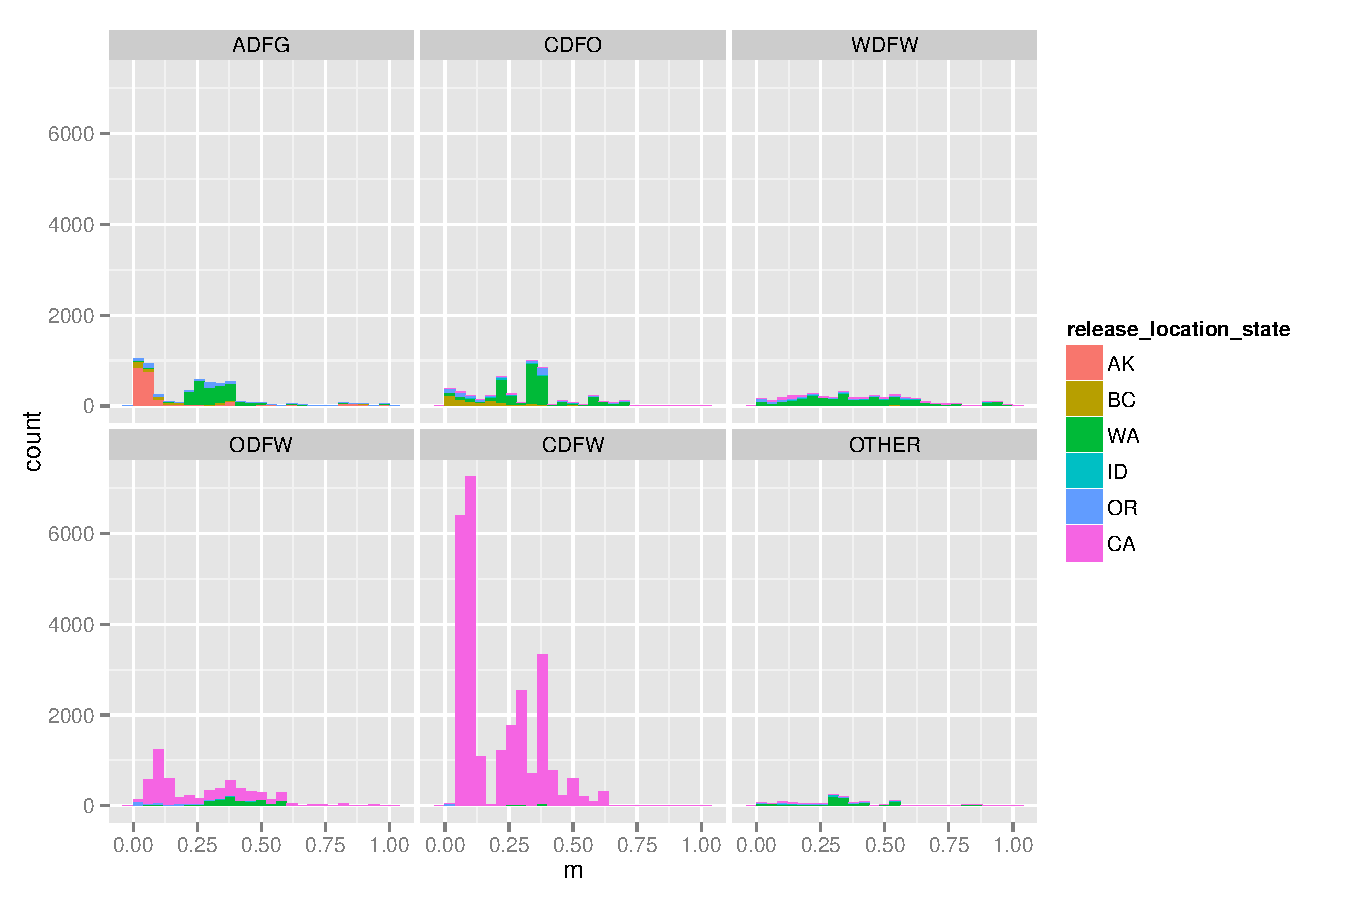
\includegraphics[width = \textwidth]{./images/m_histo_chinook.pdf}
\caption{Histograms showing the number of recoveries having different values of $m$.  The different
panels show recoveries by different agencies.  The recoveries are colored according to the 
state of their release.}
\end{figure}
  
\subsection{Fraction of families successfully tagged}
It is clear that keeping the successful tagging rate of families as high as possible is important for PBT.  One important
point this raises is the great advantage achieved if using a sufficient number of markers that single-parent
parentage assignments can be made accurately.  Figure~\ref{fig:succ_rate} shows the fraction of families tagged as a 
function of the fraction of individual parent genotypes successfully genotyped when parentage is done on the basis
of single parents or parent pairs.  
\begin{figure}
\centering
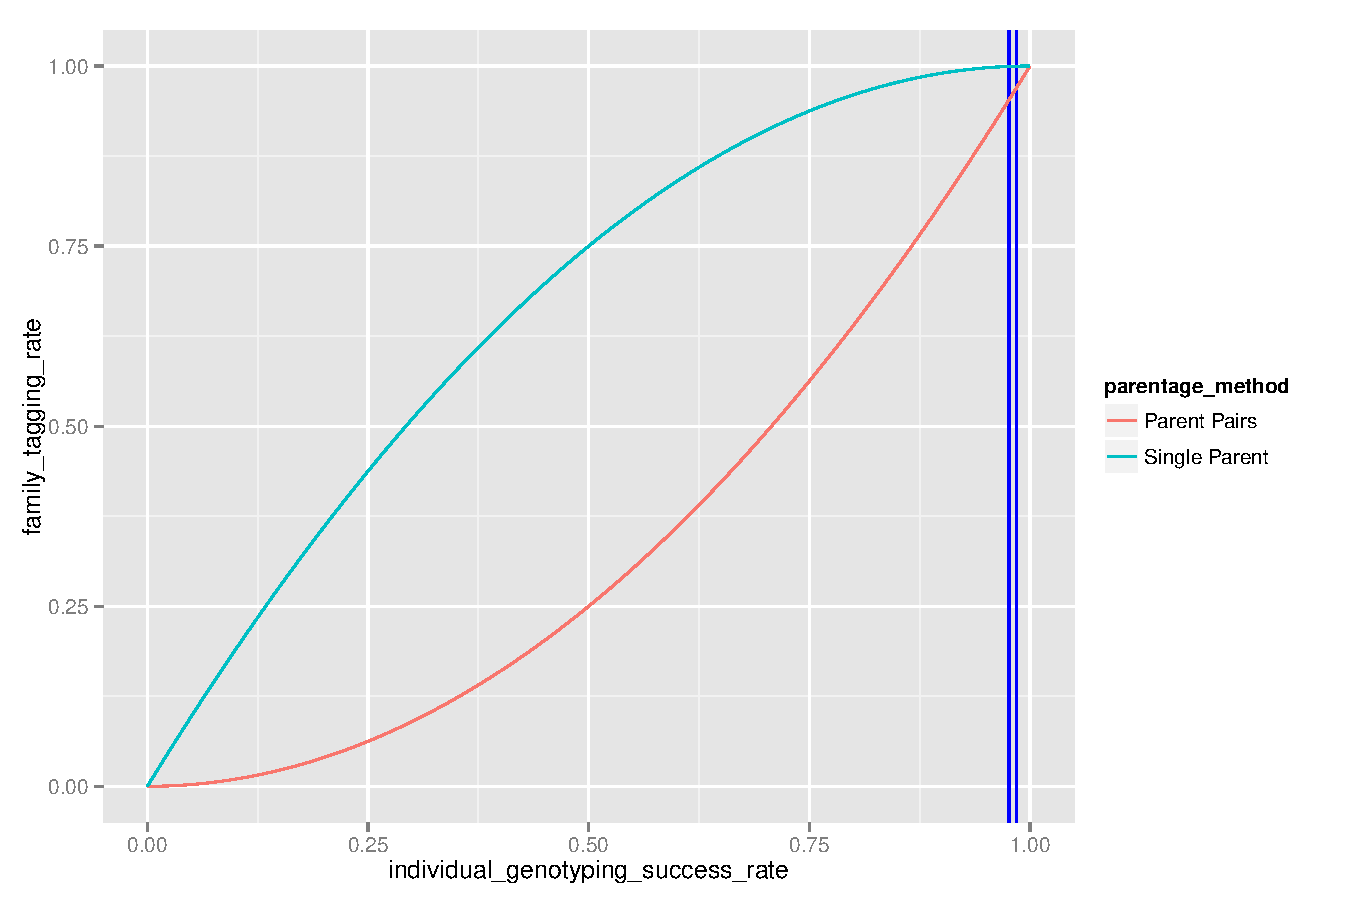
\includegraphics[width = \textwidth]{images/succ_rate.pdf}
\caption{Expected family tagging rates as a function of the rate of successful individual genotyping
under two methods of parentage assignment---single parent and parent pair assignment.  Vertical blue lines
depict the genotyping success rates achieved over 5 years in Chinook and steelhead in the Snake River
PBT program.  }
\end{figure}

If one can only make parent-pair assignments accurately, then the number of successfully-tagged
families decrease quickly when a few individuals are unsuccessfully genotyped.  However, if single-parent assignments
are possible, the family tagging rate decreases much more  slowly because only one parent needs be successfully genotyped
to tag the family.  For example, even if the individual genotyping success rate is as low as 0.86, the family tagging rate
is still expected to exceed 0.98.  

The most comprehensive data available individual genotyping success rate comes from the Snake River basin where a PBT program has been 
ongoing in Chinook and steelhead for over 6 years.  From 2009 to 2013, 43,770 of 44,468 total chinook were successfully genotyped---a success
rate of 98.43\%.  During the same period 26,908 of 27,565 steelhead (97.62\%) were successfully genotyped.  The expected family tagging
rates in these program, using parent-pair assignments is thus 0.969, and 0.953, respectively.  Using single parent assignments, 
the expected family tagging rates would both be 0.9998 and 0.9994.  

\section{Conclusions}

Variance in PBT tagging rates is most likely to decrease accuracy of PBT-based estimates of expanded fish numbers
when all four of the following conditions coincide:
\begin{enumerate}
\item Release groups are composed of offspring of fewer than 30 families,
\item The $N_b/(2S)$ ratio in the hatchery is lower than 0.7,
\item A fraction higher than 50\% of all the fish from a release group in a fishery are expected to be sampled,
\item The genotyping success rates is low enough that fewer than 96\% of families are successfully tagged.
\end{enumerate}
A review of these quantities in existing programs suggest that condition~1 is often encountered, 2 is usually encountered, 3 is infrequently 
encountered, and most importantly, long-term ongoing programs have demonstrated that genotyping success rates can be maintained 
at high levels.

This analysis indicates that careful sampling and tissue handling protocols to ensure high genotyping success and the use of sufficient markers to allow
accurate single parent assignment would reduce PBT tag rate variance and its practical consequences to negligible proportions.

\bibliography{../bibstuff/pbtfeas}
\bibliographystyle{mychicago}
 \end{document}
